\chapter{Descripción del Trabajo}
\label{cap:descripcionTrabajo}
\section{Descripción de la herramienta}
\label{sec:Descripción de la herramienta}
Se desea diseñar una herramienta donde dado el usuario unas imágenes y unas configuraciones el programa pueda reconocer el texto de la imagen y detectar si existe algún error de localización de las que hemos seleccionado.

Para ello la herramienta además del programa principal, constará de dos módulos:
\begin{itemize}
	\item Modulo del OCR.
	\item Modulo del test.
\end{itemize}
\subsection{Modulo de OCR}
El modulo de OCR se encarga de todo lo relacionado con la detección de texto en imágenes y la mejora de la detección.

En este modulo se elegirá una librería de OCR para la detección de texto y tendrá principalmente dos funcionalidades: 
\begin{itemize}
	\item Entrenar modelo: Dado una fuente y un idioma, el OCR entrena un modelo especifico para esa fuente en concreta y ese idioma en concreto, mejorando así el resultado obtenido.
	\item Reconocer texto: Dado una imagen o una ruta de imagen, el OCR reconoce texto y los guarda en un archivo txt o se lo pasa al programa.
\end{itemize}
En este módulo, recibirá como entrada imágenes a reconocer y unas configuraciones:
\begin{itemize}
	\item La ruta de la imagen.
	\item La ruta del ground-truth.
	\item La ruta del modelo a utilizar.
	\item Nombre del modelo a utilizar.
\end{itemize}
Con las imágenes, pasará por un proceso de preprocesado para mejorar la calidad de la imagen en el sentido de que el OCR reconozca mejor los caractéres y generará un texto.
Ese texto antes de ser pasado como entrada al siguiente modulo será procesado otra vez para minimizar el error producido por el OCR en lo mejor posible.
Debido a la necesidad de algunos test, también se ha considerado obtener informaciones como posición del texto en la imagen en este modulo.
\subsection{Modulo de test}
El modulo de test se cargará de verificar si existe algún error de localización con el texto obtenido del OCR.

Usará como entrada, la salida del modulo de OCR y pasará por una serie de tests para verificar si existe o no algún error de localización. La salida de este modulo será el resultado de los tests indicando si ha pasado el tests y en caso negativo indicar (si es posible) donde se produce el fallo.

Con esa salida se generará un archivo json, que luego será interpretado para que sea entendible por un ser humano.
\section{Descripción de los tests}
\label{sec:Descripción de los tests}

Se elegirá unos de los tests de todos los errores comunes de localización y como se atacará ese error.Se ha elegido estos errores considerando la importancia y la relevancia con nuestra herramienta(p.ej atacar el error de audio no tiene sentido en este trabajo).

\subsection{Testing sobre solapamiento de texto }
Para resolver este problema se plantea usar el OCR para detectar las posiciones de los textos, seguido de una librería gráfica para detectar el contorno de la caja delimitadora guardado para ese texto, y obtener así sus posiciones. Comparando la posición del texto y la posición de la caja delimitadora obtenemos si el texto se está saliendo de la caja o no.

Para simplificar el test, damos algunas restricciones: 
\begin{itemize}
	\item En la imagen, el texto tiene que aparecer completamente en horizontal sin ninguna rotación sobre el eje X.
	\item Detectamos texto que sobresale por los lados.
	\item Tiene que estar resaltado y tener un claro contraste con el fondo y el texto para facilitar la detección.
	\item Debe tener una forma de caja o ventana(cuadriculada, cuadriculada redondeada). No sirve, por ejemplo, un bocadillo en forma de nube.
\end{itemize} 
La salida indicará si existe o no solapamiento en la imagen.

\subsection{Testing sobre detección de placeholders}
Este es un error que no se describió en el apartado de errores comunes de localización\ref{sec:Errores de localizacion}, es un error que he experimentado como usuario y que aparece en muchas ocasiones por lo que he decido evaluarlo. Este error aparece cuando por algún error del desarrollador aparecen placeholders en la pantalla del juego en vez del texto(p.ej si en el juego me llamo ``pepe'', en vez de aparecer en el dialogo ``Hola pepe'', aparece un ``Hola \%*player\_name*\%'').
Para resolver este problema se plantea con la antelación de saber cual es el placeholder usado, hacer una búsqueda del placeholder en el texto reconocido por el OCR.

Se tiene en cuenta las siguientes restrincciones:
\begin{itemize}
	\item El placeholder es formado por al menos un carácter de apertura y al menos un carácter de cierre. Puede tener más de un carácter en ambos lados.
	\item Todo lo que este entre la cadena de apertura y cadena de cierre se considera placeholder sin importar el número de palabras que hay dentro.
	\item Existe un solo tipo de placeholder, de momento no soporta la detección de múltiples tipos de placeholders.
\end{itemize}
La salida indicará si existe placeholder en la imagen y la posición en la que se encuentra para una mejor búsqueda por parte del personal de QA.
\subsection{Testing sobre truncamiento de texto}

Para resolver este problema se plantea obtener la cadena esperada y la cadena reconocida por el OCR. Se compara la longitud de ambas cadenas, si la longitud es la misma, entonces no existe truncamiento. En caso contrario, se hará comparaciones palabra a palabra buscando la existencia de subcadenas (p.ej ``ment'' es subcadena de ``mente''), en caso de encontrar subcadenas, entonces existe un truncamiento. Si no se encuentran subcadenas, significa que son diferentes frases por lo que sería otro tipo de error.

La restricción para este test:
\begin{itemize}
	\item Es necesario tener la cadena esperada.
\end{itemize}
La salida indicara si existe o no truncamiento en el texto.

	
\section{Librerías de OCR (Optical Character Recognition)}
\label{sec:Seleccion de libreria de OCR}
Durante el desarrollo de este trabajo, se evaluaron varias herramientas de OCR para seleccionar la más adecuada para nuestras necesidades. Las herramientas probadas fueron Ocropus	\footnote{(repositorio github de Ocropus) \url{https://github.com/ocropus-archive/DUP-ocropy} }, EasyOCR	\footnote{(repositorio github de EasyOCR) \url{https://github.com/JaidedAI/EasyOCR} } y Tesseract	\footnote{(repositorio github de Tesseract) \url{https://github.com/tesseract-ocr/tesseract} }. A continuación, se describe brevemente cada una de ellas.
\begin{enumerate}
	\item \textbf{OCRopus}
	Es un sistema de OCR basado en redes neuronales con un enfoque modular.
	Principalmente esta disponible para Linux. Proporciona diferentes módulos para la binarización, segmentación, generación del ground-truth y el entreno del modelo.
	Una de las razones por la que esta herramienta fue descartado es que el lenguaje de programación principal con la que trabaja es \emph{python} y en nuestro proyecto trabajamos principalmente con \emph{C++}. Además la última actualización de esta librería fue en 16 de Diciembre de 2017
	
	\item \textbf{EasyOCR}
	EasyOCR es una biblioteca de reconocimiento óptico de caracteres (OCR) desarrollada en Python que facilita la extracción de texto de imágenes y documentos. Diseñada con el objetivo de ser fácil de usar y accesible, una de las características de EasyOCR es que es capaz de reconocer texto en más de 80 idiomas y soporta múltiples scripts, lo que la convierte en una herramienta versátil para diversas aplicaciones.
	Proporciona gran variedad de modelos entrenados y también ofrece la opción de entrenar tu propio modelo.
	
	La herramienta en resumen se adapta muy bien a nuestras necesidades. El único problema esta en el idioma de programación con la que trabaja , al igual que OCRopus , EasyOCR está implementada con \emph{python} y nosotros con \emph{C++}.
	
	\item \textbf{Tesseract}
	
	Tesseract es una biblioteca de (OCR) de código abierto que se utiliza para convertir imágenes de texto en texto editable. Originalmente desarrollado por Hewlett-Packard en la década de 1980, Tesseract fue liberado como software de código abierto en 2005 y ha sido mantenido y mejorado por la comunidad, particularmente por Google, que ha contribuido significativamente a su desarrollo.
	
	Al igual que EasyOCR una de las características más destacadas de Tesseract es su capacidad para reconocer texto en múltiples idiomas y alfabetos, soportando más de 100 idiomas de forma nativa. Esto lo convierte en una herramienta versátil para aplicaciones globales que requieren la extracción de texto de documentos escritos en diferentes lenguas.
	
	Tesseract utiliza técnicas avanzadas de aprendizaje profundo y redes neuronales, lo que le permite alcanzar altos niveles de precisión en el reconocimiento de texto. Su arquitectura se basa en el uso de modelos de aprendizaje profundo entrenados con grandes conjuntos de datos, lo que mejora continuamente su rendimiento en diversas condiciones.
	
	El motor puede integrarse fácilmente en aplicaciones de procesamiento de imágenes y visión por computadora. Tesseract se utiliza comúnmente en combinación con bibliotecas como OpenCV para preprocesar imágenes antes de la etapa de reconocimiento, lo que mejora la precisión de los resultados.
	
	Además, Tesseract ofrece una API en varios lenguajes de programación, lo que facilita su integración en diferentes entornos de desarrollo y una de ellas es C++, por lo que esta herramienta cumple con todos los requisitos para nuestro proyecto y es la razón por la que hemos optado por Tesseract.
\end{enumerate}
\subsection{Pruebas y resultados de los OCR}
En esta sección se hará una evaluación de los distintos OCRs para elegir la más conveniente para nuestra herramienta.
La evaluación se hará sobre las librerías de Tesseract, EasyOCR y Ocropus, son estas elegidas por su disponibilidad gratuita.

El objetivo de la evaluación es elegir el OCR que mejor se adapte a nuestras necesidades, lo que resalta la importancia de la precisión del OCR.
Para poder medir esa precisión, tendremos en cuenta el CER(\textit{Character Error Rate}). Además el tiempo también es un factor importante que tendremos en cuenta.

Según \cite{CER} el CER(\textit{Character Error Rate}) es una métrica usada comúnmente para evaluar la precisión de un sistema de reconocimiento de caracteres (OCR) u otros sistemas que transcriba texto. El valor se obtiene calculando el número de errores a nivel de carácter dividido por el número total de caracteres en el texto de referencia.
Los errores pueden ser debidos a:
\begin{enumerate}
	\item Sustituciones: Un carácter incorrecto reemplaza a uno correcto.
	\item Inserciones: Aparece un carácter extra que no debería estar.
	\item Eliminaciones: Falta un carácter que debería estar presente.
\end{enumerate}
La fórmula general para calcular el CER es:
	
	$CER = \frac{S+D+I}{N} $ 

Donde:

S es el número de sustituciones.

D es el número de eliminaciones.

I es el número de inserciones.

N es el número total de caracteres en el texto de referencia.

El CER se expresa como un valor entre 0 y 1 (o como porcentaje), donde 0 significa que no hubo errores (transcripción perfecta) y 1 (o 100) indica que todos los caracteres son incorrectos.

La metodología seguida para la evaluación es la siguiente:

\begin{enumerate}
	\item Se hará la evaluación de forma independiente con las 3 librerías de OCR. Tesseract, EasyOCR y Ocropus.
	\item Se ha elegido 13 imágenes nombrados del 1 al 13 siendo la imagen 1(figura \ref{fig:1.png}) el más simple y el 13(figura \ref{fig:13.png}) el más complejo. Para la clasificación de simplificad de las imágenes se ha tenido en cuenta el número de caracteres a reconocer y la complejidad del fondo, entre ellas, el contraste y el número de geometrías.
	Las imágenes se pueden encontrar en el repositorio del trabajo\footnote{(Repositorio github con las imágenes de evaluación)\url{https://github.com/Dewo2000/TFG-2024-2025/tree/main/OCRTests/images}}.
		\begin{figure}[H]
		\centering
		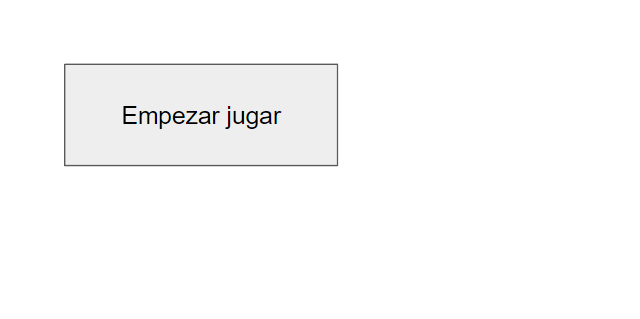
\includegraphics[width = 1\textwidth]{Imagenes/Evaluacion_OCR/1.png}
		\caption{1.png}
		\label{fig:1.png}
	\end{figure}
		\begin{figure}[H]
		\centering
		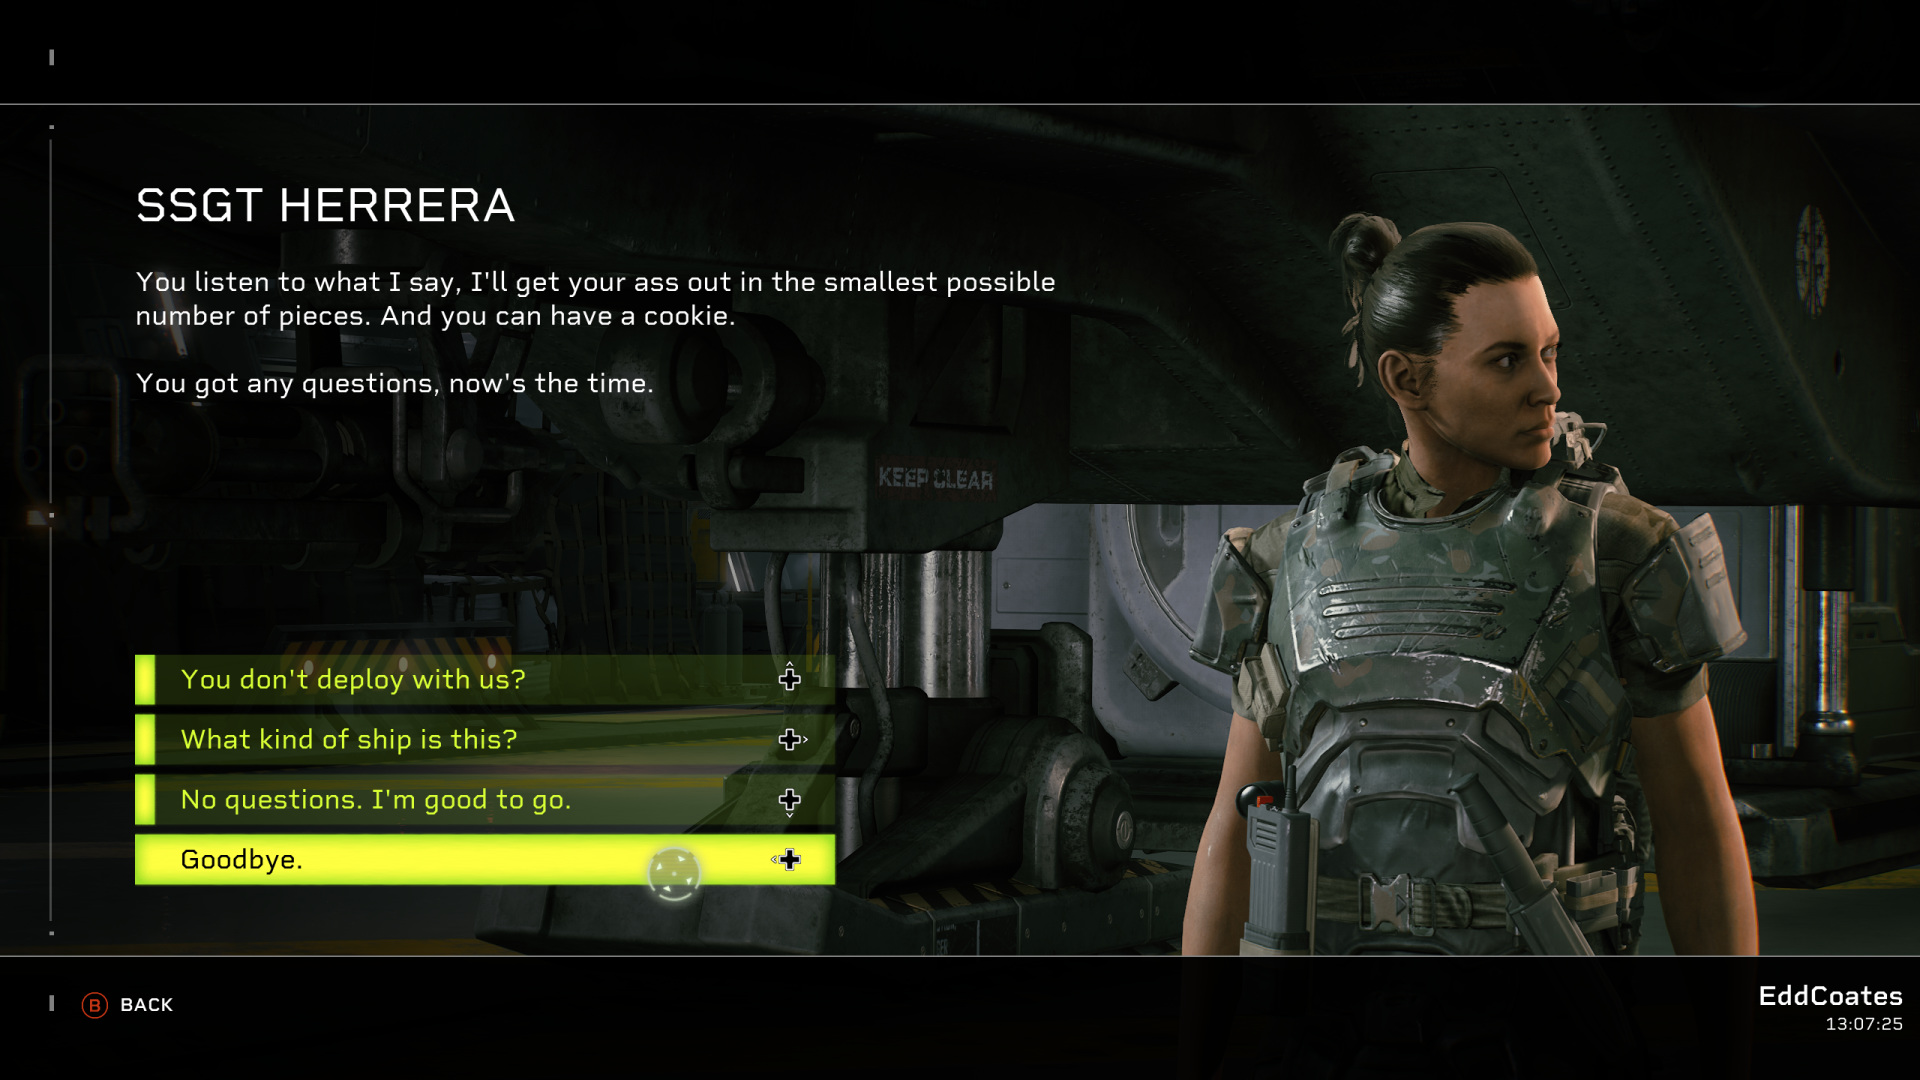
\includegraphics[width = 1\textwidth]{Imagenes/Evaluacion_OCR/13.png}
		\caption{13.png}
		\label{fig:13.png}
	\end{figure}
	\item Cada imagen será procesadas por el OCR utilizando el modelo por defecto de cada una de ellas.  
	\item Se utiliza la libreria Jiwer\footnote{(Jiwer Usage)\url {https://jitsi.github.io/jiwer/usage/}} en python para los cálculos de CER.
	\item Se ejecutará 6 veces el proceso de reconocimiento de cada OCR para sacar el tiempo medio de cada una.
\end{enumerate}


En los resultados de los ocr se encontrará un valor llamado CER medio, este valor se obtiene calculando el número total de errores a nivel de carácter encontrado en toda la batería de prueba divido entre el número total de caracteres de toda la batería de prueba.

Los resultados de los OCRs son las siguientes:
	\begin{table}[H]
		\centering
		\caption{Resultado de CER de los OCR (Redondeado a 3 decimales)}
		\begin{tabular}{llll}
			\textbf{Imagen} & \textbf{Tesseract} & \textbf{EasyOCR} &\textbf{Ocropus} \\
		1  & 0.000 & 0.000 & 0.000 \\
		2  & 0.063 & 0.281 & 0.406 \\
		3  & 0.538 & 0.212 & 0.538 \\
		4  & 0.043 & 0.109 & 0.978 \\
		5  & 0.289 & 0.086 & 0.719 \\
		6  & 0.025 & 0.025 & 0.700 \\
		7  & 0.750 & 0.000 & 1.417 \\
		8  & 0.935 & 0.652 & 0.870 \\
		9  & 0.721 & 0.256 & 0.744 \\
		10 & 1.000 & 0.857 & 8.286 \\
		11 & 0.050 & 0.150 & 2.550 \\
		12 & 0.352 & 0.055 & 0.834 \\
		13 & 0.230 & 0.337 & 0.881 \\
			\textbf{CER medio} & \textbf{0.384}& \textbf{0.232} & \textbf{1.456}\\
		\end{tabular}
		\label{table:TesseractResult}
	\end{table}
	\begin{table}[H]
	\centering
	\caption{Resultado de OCR en tiempo(ms)}
	\begin{tabular}{llll}
		\textbf{Iteración} & \textbf{Tesseract}& \textbf{EasyOCR}& \textbf{Ocropus} \\
		1  & 5539   & 204625 & 86213  \\
		2  & 5580   & 223809 & 90172  \\
		3  & 5539   & 216701 & 88290  \\
		4  & 5720   & 238900 & 83278  \\
		5  & 5602   & 216791 & 87810  \\
		6  & 5571   & 204502 & 88789  \\
		\textbf{Tiempo medio} & \textbf{5591}&\textbf{217554}&\textbf{87425} \\
		\end{tabular}
		\label{table:TesseractResultTime}
	\end{table}


Como podemos ver en los resultados, todos los OCRs han podido reconocer de forma exacta la imagen más simple y que todos han caido en la imagén 10. En cuanto las otras imágenes podemos observar que unas lo reconoce mejor Tesseract y otras EasyOCR por lo que ambos producen buenos resultados, en cuanto Ocropus, sus resultados ya no son tan buenos en comparación con las otras dos por lo que queda descartado. Aunque EasyOCR obtiene un mejor CER medio en los resultados (0.23) que Tesseract (0.38), Tesseract es muchísimo más rápido que EasyOCR teniendo un 211936 milisegundo de adelanto que equivale a 3 minutos y 50 segundos aproximadamente. Por tanto decidimos seguir en adelante con Tesseract.



\section{Mejoras en el reconocimiento de texto en imágenes}
\label{sec:Mejoras en el reconocimiento}
Como podemos notar en los resultados del apartado anterior, la imagen 10 ha sido un reto para el CER de los OCRs, esto es debido a que el OCR reconoce como carácter geometrías del fondo y produce basura.Para solucionar esto, se plantea aplicar preprocesamiento a las imágenes y la limpieza del resultado usando distancia Levenshtein para mejorar la precisión del texto obtenido por el OCR disminuyendo el CER.

Para obtener más información sobre aquellos factores o características de las imágenes que puedan afectar al rendimiento y efectividad de la herramienta de OCR, se ha clasificado las imágenes en 5 categorías diferentes. La clasificación se ha hecho a ojo humano de forma subjetiva.
\begin{enumerate}
	\item Fondos simples(F.Simple)(Figura \ref{fig:Fsimple}). Imágenes donde la cantidad de geometrías del fondo son pocas o fáciles de reconocer(no se confunde con los caractéres).
		\begin{figure}[H]
		\centering
		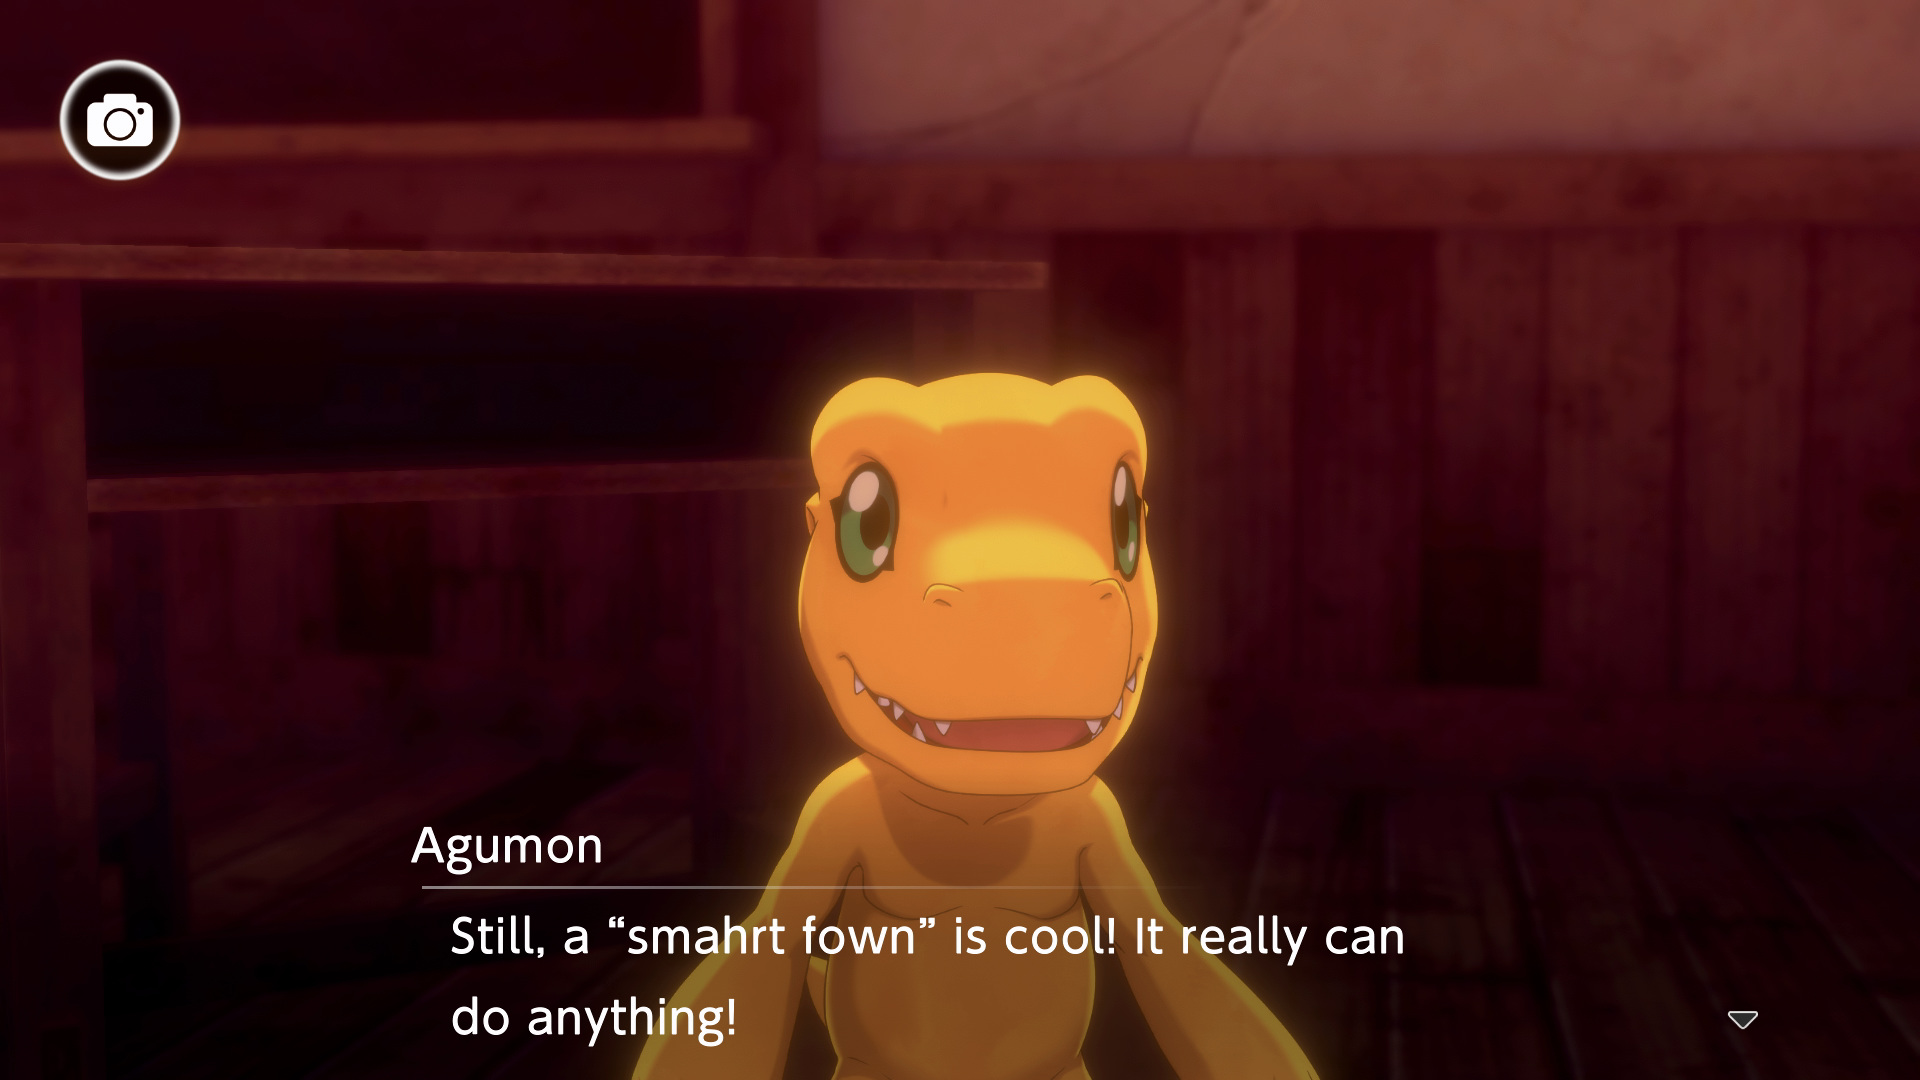
\includegraphics[width = 0.5\textwidth]{Imagenes/OCR/Simple.png}
		\caption{Ejemplo imagen fondos simples }
		\label{fig:Fsimple}
	\end{figure}
	
	\item Fondos complejos(F.Complejo)(Figura \ref{fig:Fcomplejo}). Imágenes donde la cantidad de geometrías del fondo son muchas o difíciles de reconocer(fácil de confundirse con los caractéres).
		\begin{figure}[H]
		\centering
		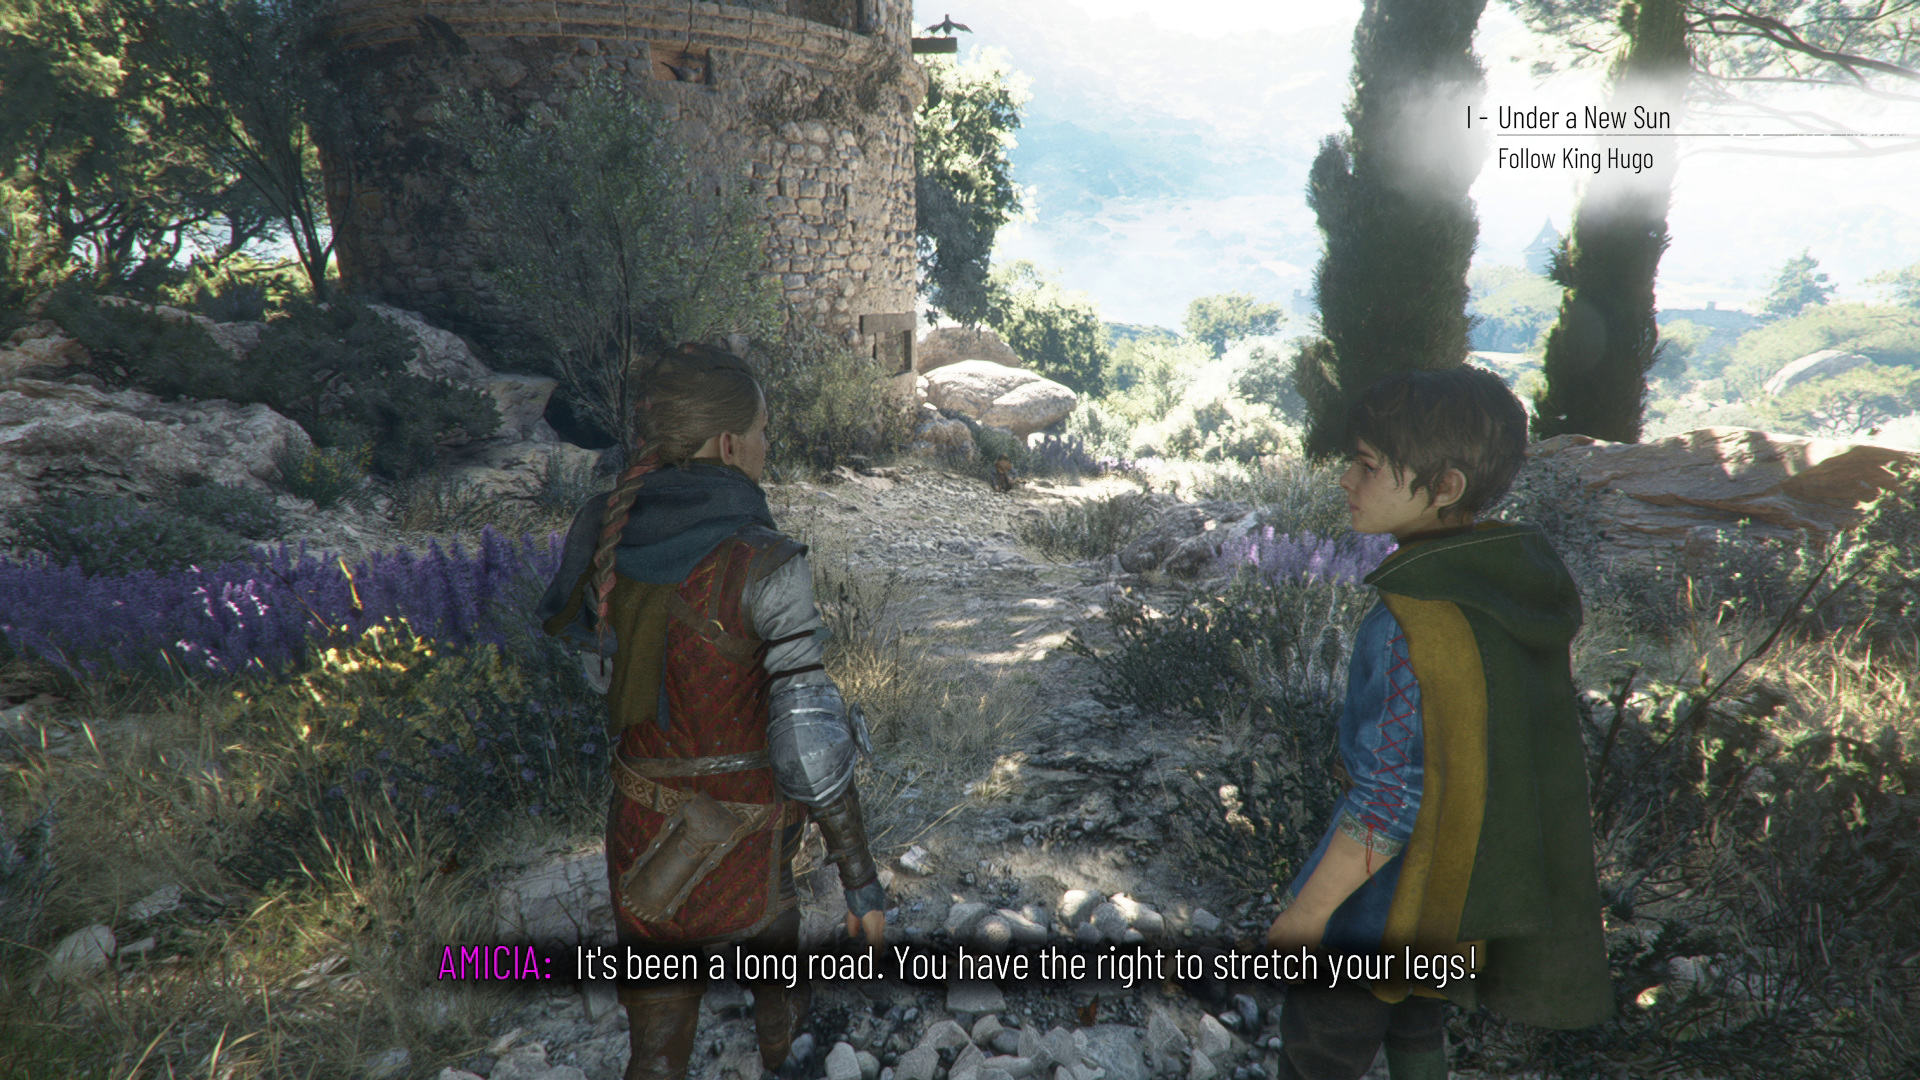
\includegraphics[width = 0.5\textwidth]{Imagenes/OCR/Complejo.png}
		\caption{Ejemplo imagen fondos complejos }
			\label{fig:Fcomplejo}
	\end{figure}
	\item PixelArt(PixelArt)(Figura \ref{fig:Pixelart}). Imágenes donde el fondo y las letras tiene un estilo pixelart. Como las imágenes son píxeladas(cuadrado de color que forman formas y texto), supone un reto para el OCR.
		\begin{figure}[H]
		\centering
		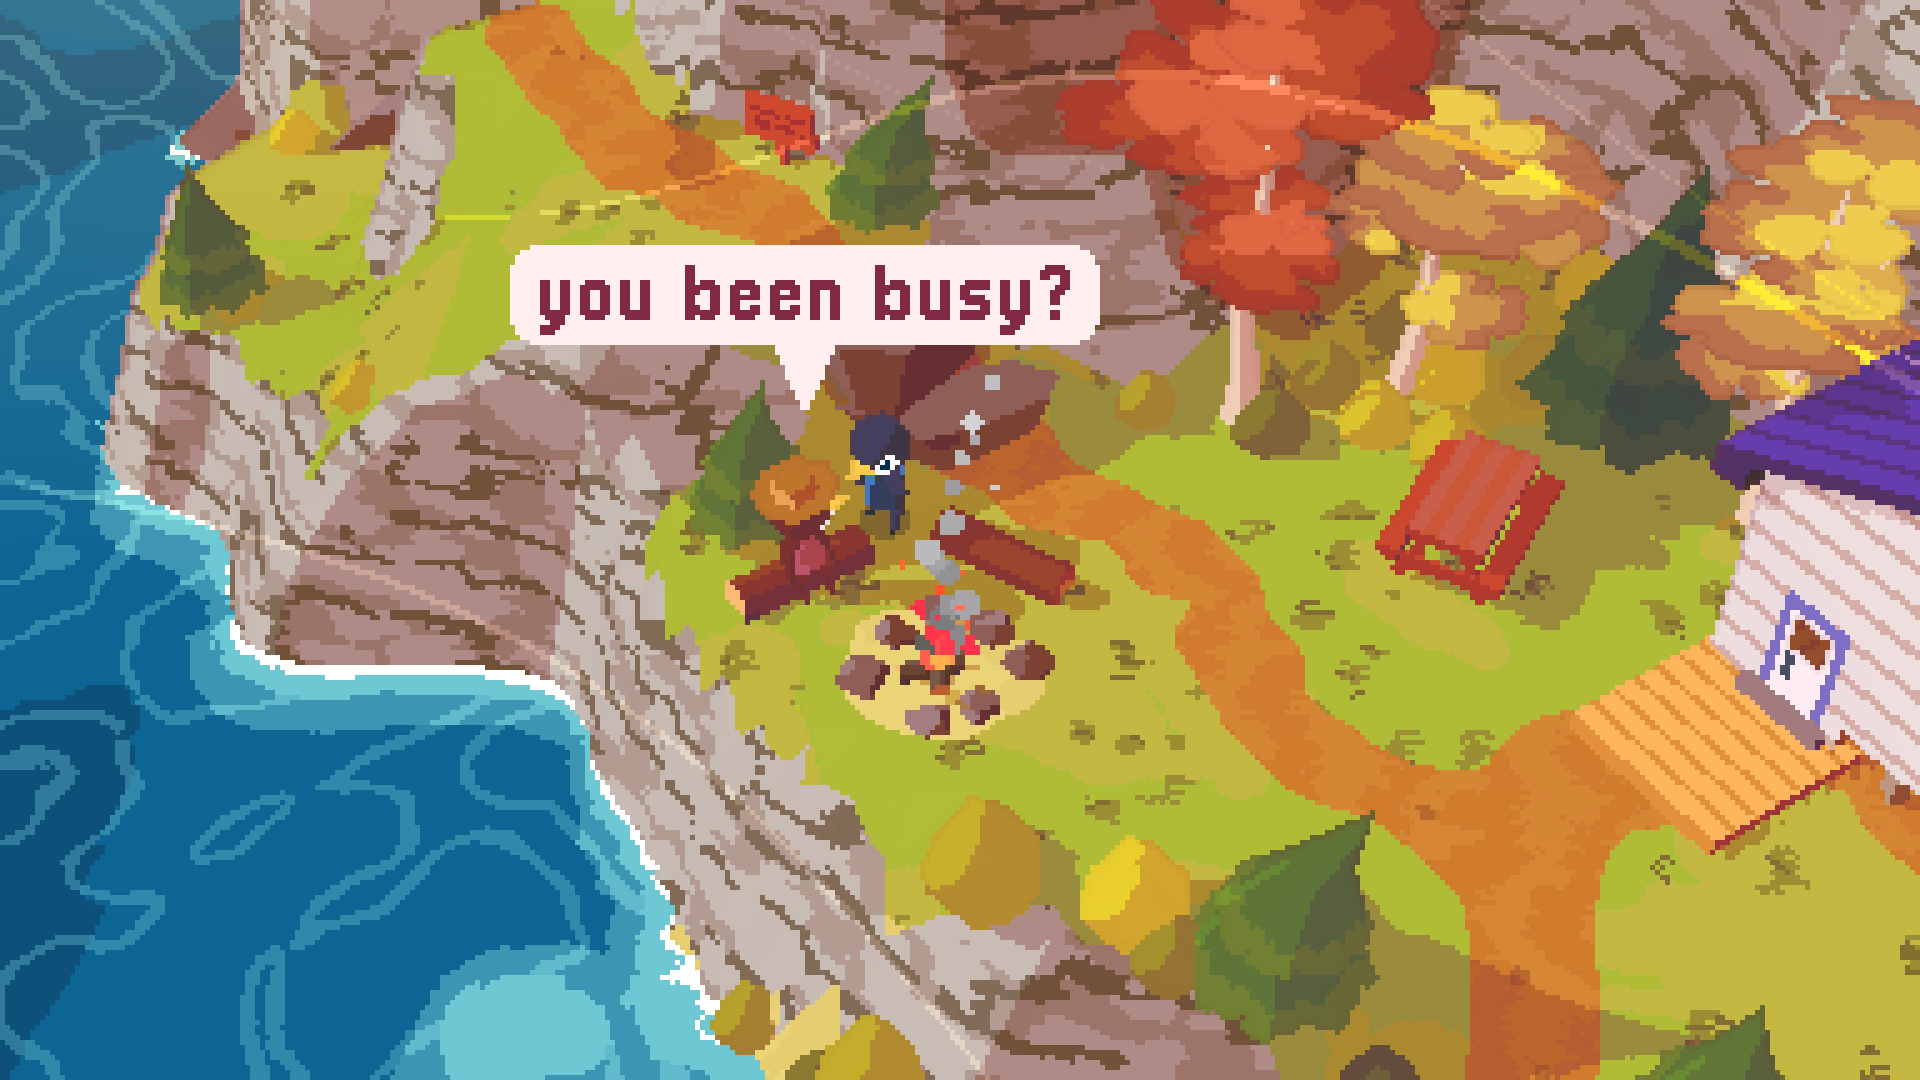
\includegraphics[width = 0.5\textwidth]{Imagenes/OCR/Pixel.png}
		\caption{Ejemplo imagen PixelArt }
		\label{fig:Pixelart}
	\end{figure}
	\item Texto en bocadillos(TxtBoc)(Figura \ref{fig:TxtBoc}). Imágenes donde el texto a reconocer se situa en un bocadillo y que el color del bocadillo tiene un alto contraste con el fondo.
		\begin{figure}[H]
		\centering
		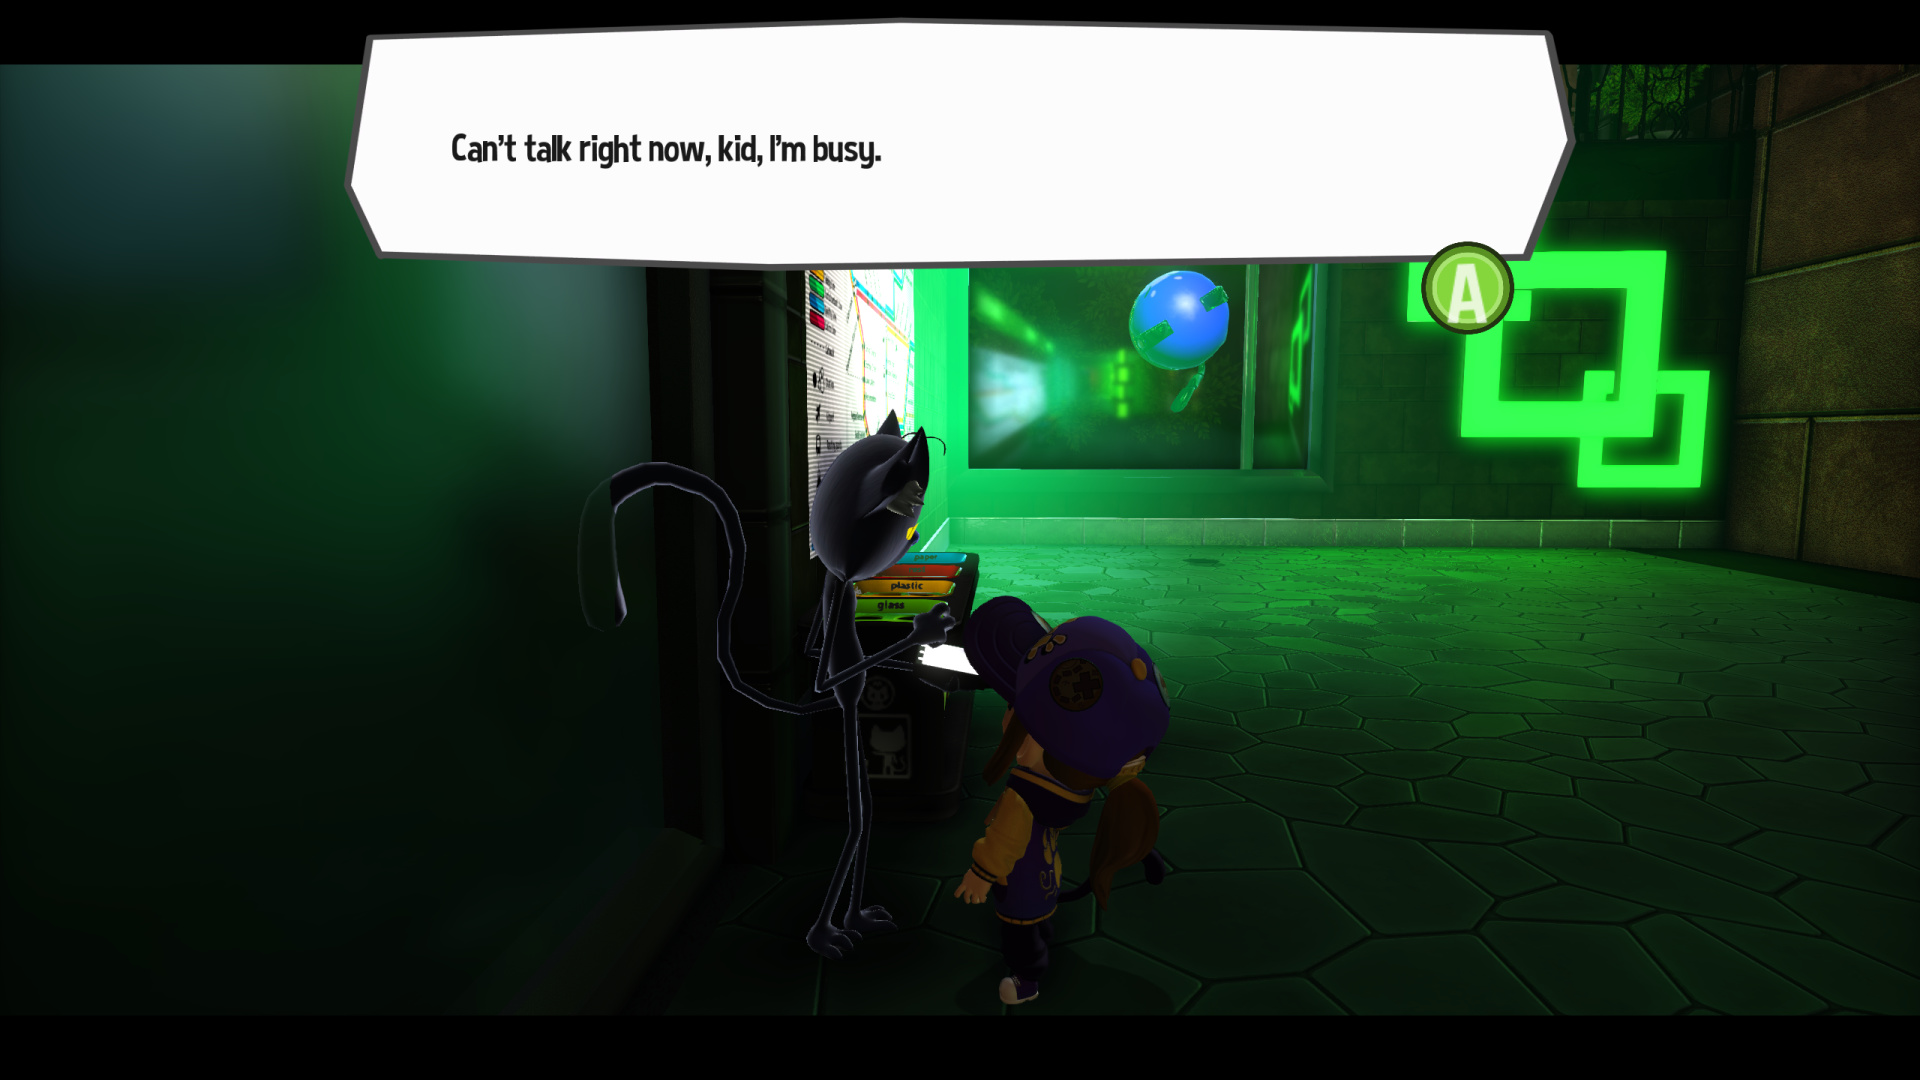
\includegraphics[width = 0.5\textwidth]{Imagenes/OCR/Boc.png}
		\caption{Ejemplo imagen de texto en bocadillo }
		\label{fig:TxTBoc}
	\end{figure}
	\item Texto en bocadillos con poca diferenciación con el fondo(TxtBoc2)(Figura \ref{fig:TxtBoc2}).Imágenes donde el texto a reconocer se situa en un bocadillo y que el color del bocadillo tiene un contraste medio o bajo con el fondo.
		\begin{figure}[H]
		\centering
		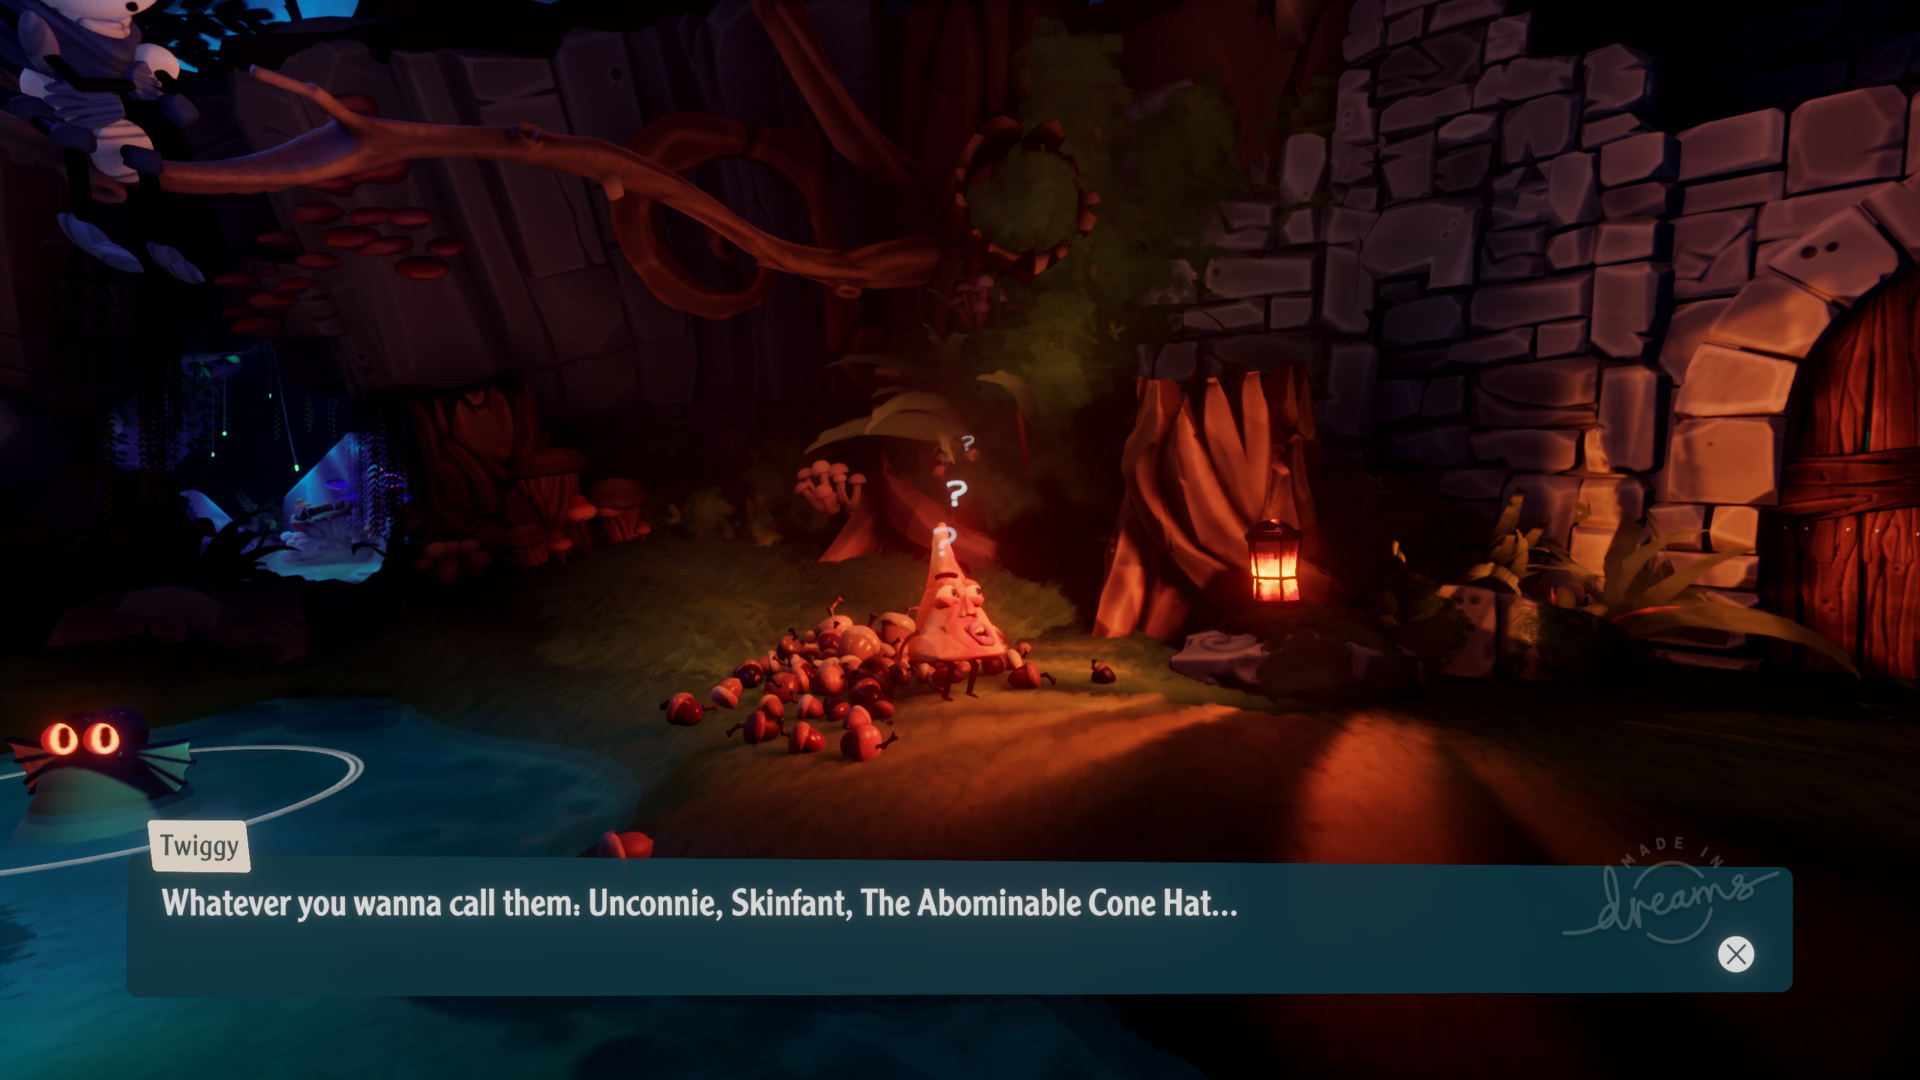
\includegraphics[width = 0.5\textwidth]{Imagenes/OCR/Boc2.png}
		\caption{Ejemplo imagen de texto en bocadillos con poca diferenciación con el fondo }
		\label{fig:TxtBoc2}
	\end{figure}
\end{enumerate} 


El preprocesamiento de imágenes consiste en aplicar técnicas que modifican las imágenes para que sea más fácil de reconocer por una OCR el texto existente.
Para saber que técnicas mejoran el reconocimiento, se ha ido probando con cada una de ellas en el manual de \cite{OpenCVProcessing}, obteniendo los resultados e identificando aquellas técnicas que ayuda a mejorar el CER medio.
Las técnicas probadas son las siguientes:

\begin{enumerate}
	\item Escala de grises(Figura \ref{fig:EscalaGrises}):
	Convierte una imagen a un formato de un solo canal, representando solo la intensidad de luz. Es útil para simplificar y reducir la cantidad de datos cuando el color no es relevante.
	\begin{figure}[H]
		\centering
		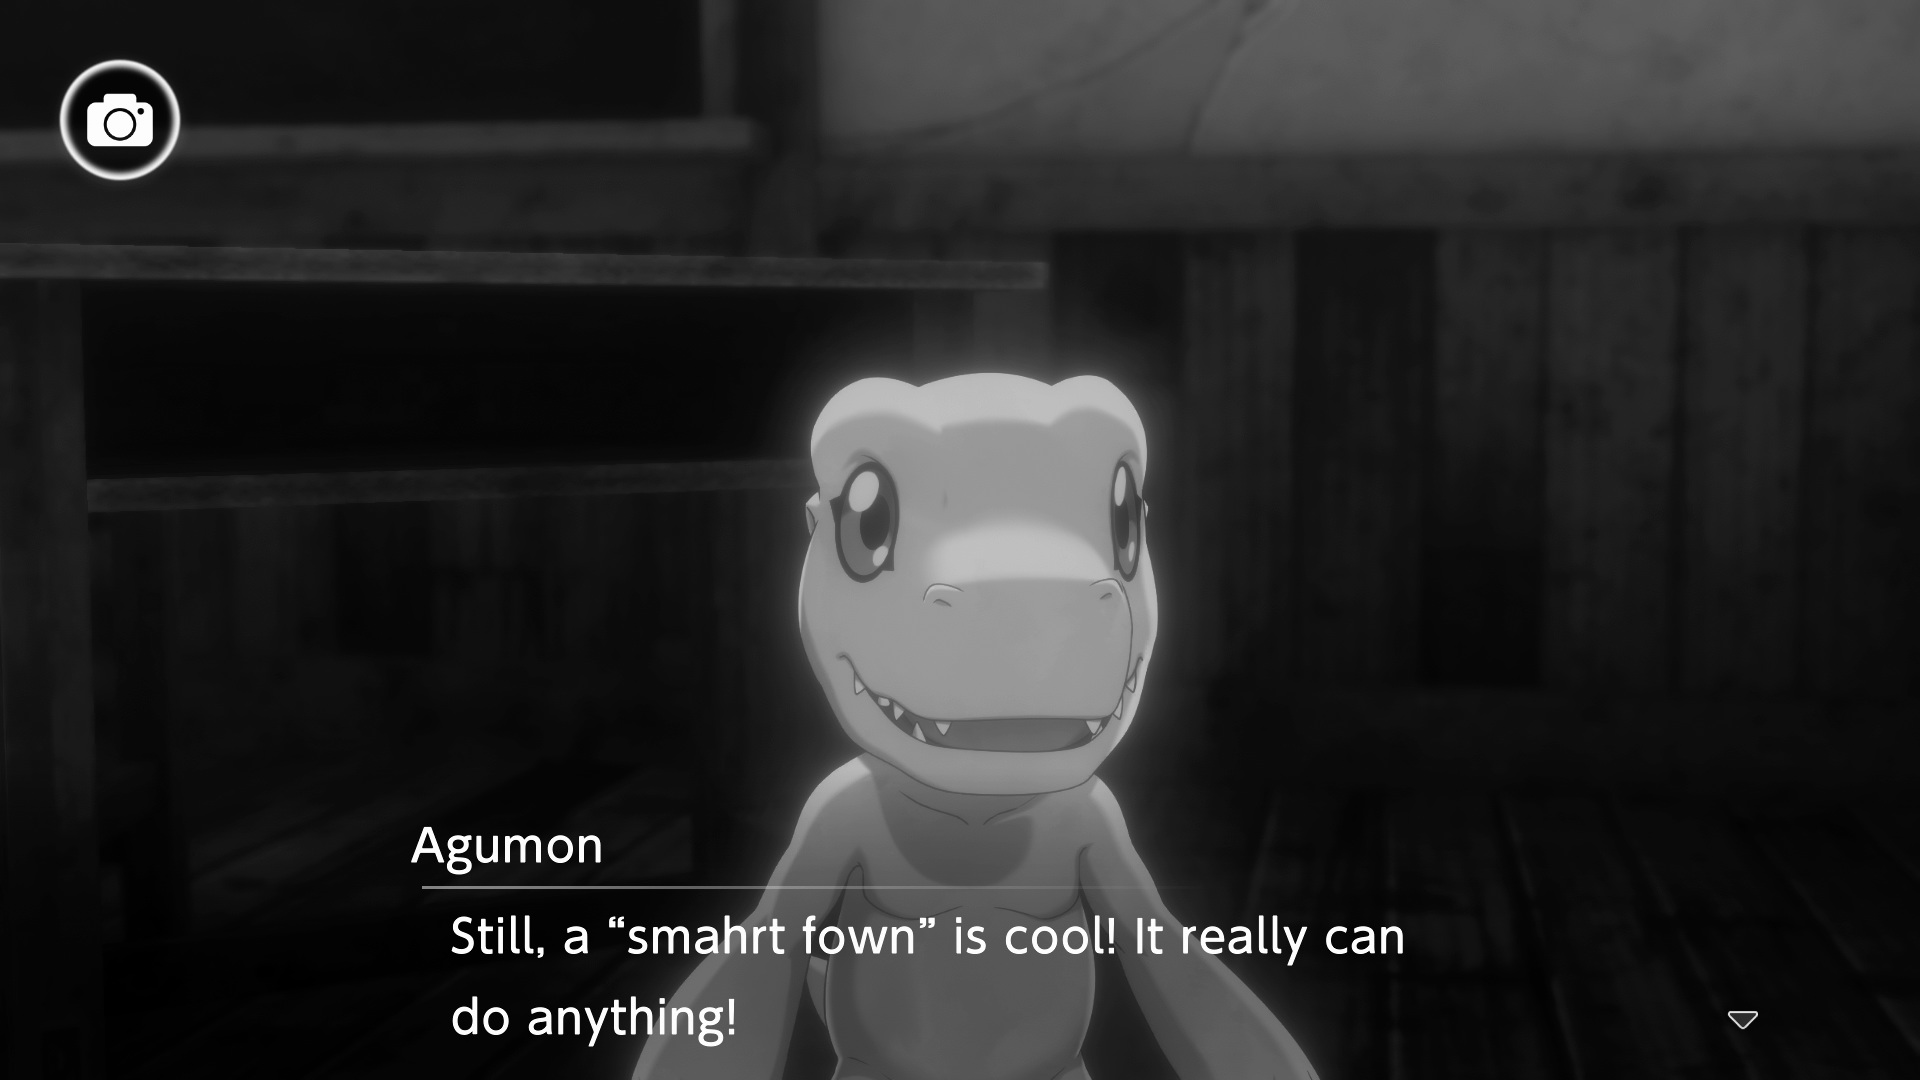
\includegraphics[width = 0.5\textwidth]{Imagenes/Preprocesado/1.png}
		\caption{Imagen a escala de grises}
		\label{fig:EscalaGrises}
	\end{figure}
	\item Aumentar contraste(Figura \ref{fig:Contraste}): 
	Mejora la diferencia entre las áreas claras y oscuras en una imagen, lo que facilita la detección de detalles.
		\begin{figure}[H]
		\centering
		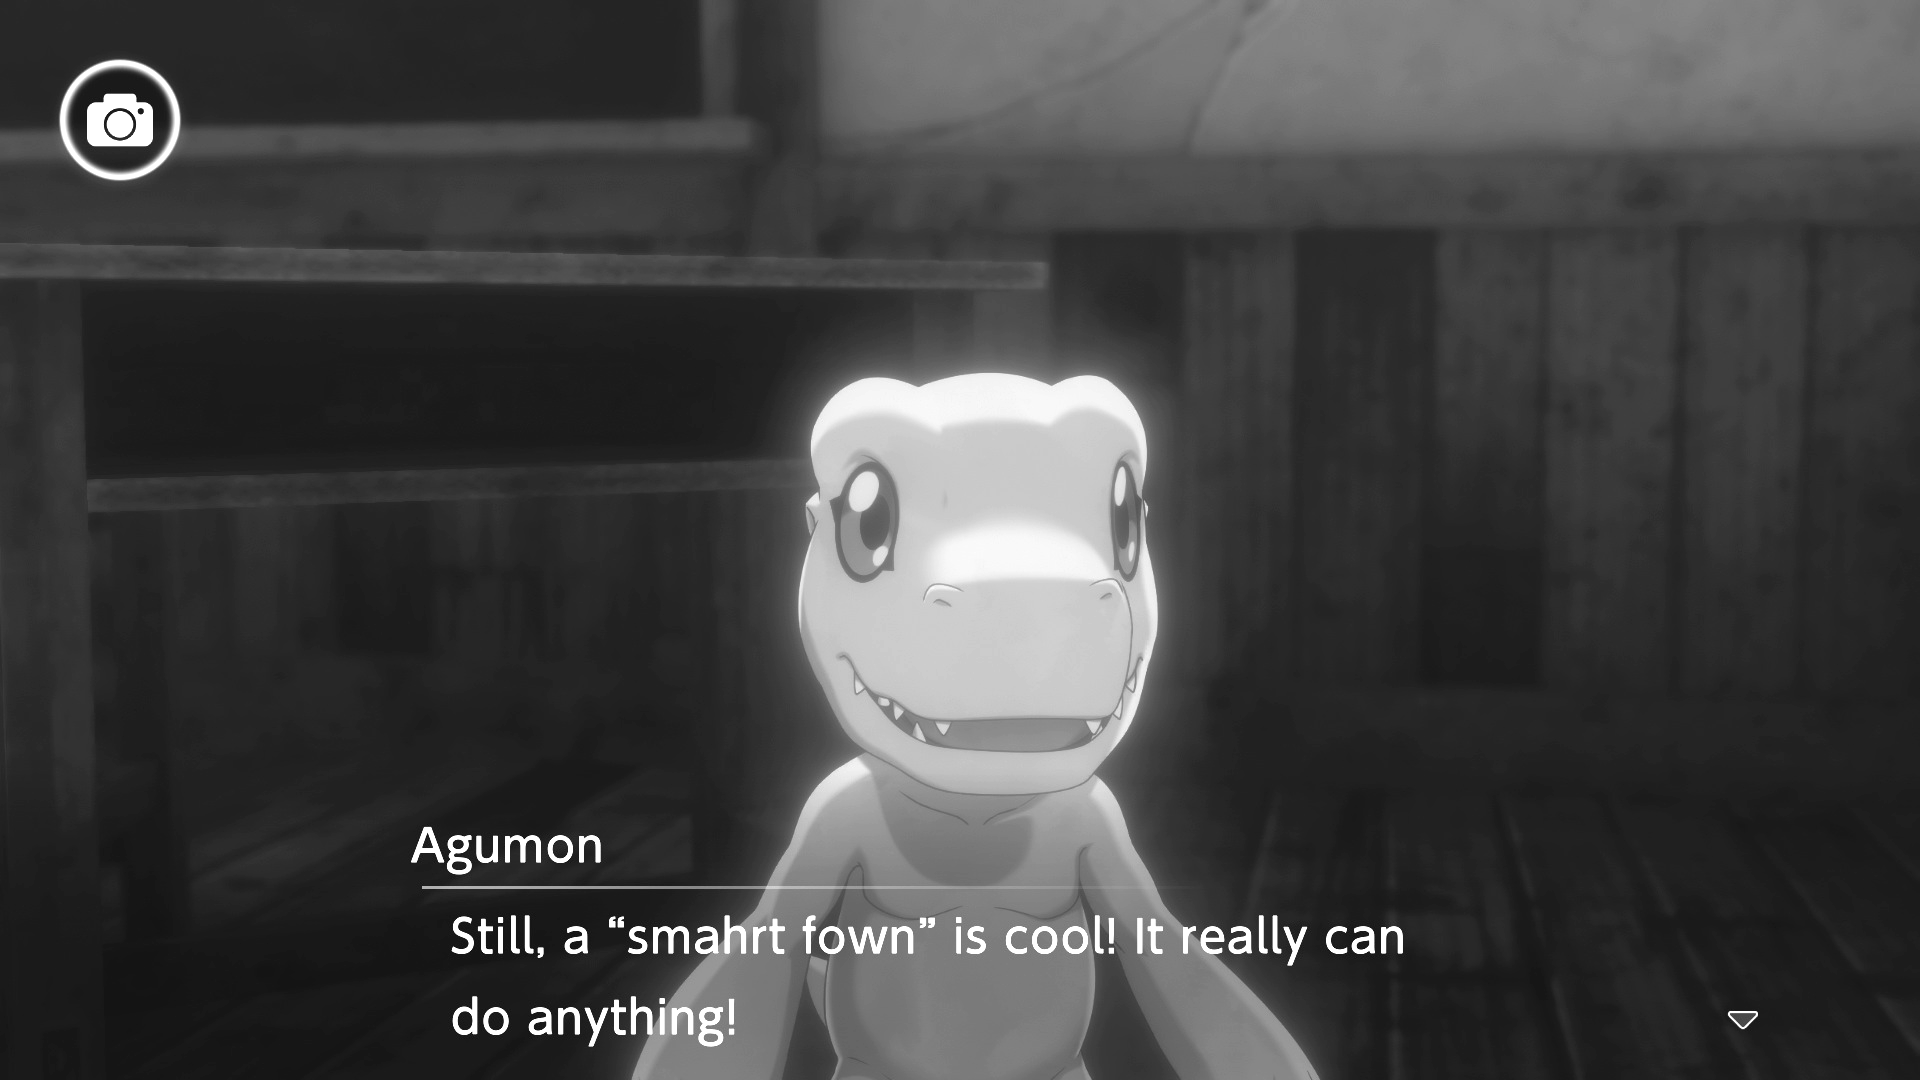
\includegraphics[width = 0.5\textwidth]{Imagenes/Preprocesado/2.png}
		\caption{Imagen con aumento de contraste}
		\label{fig:Contraste}
	\end{figure}
	\item Ecualización del histograma(Figura \ref{fig:Histograma}):
	Ajusta el contraste de la imagen extendiendo la distribución de los niveles de gris, mejorando el rango dinámico y resaltando los detalles.
		\begin{figure}[H]
		\centering
		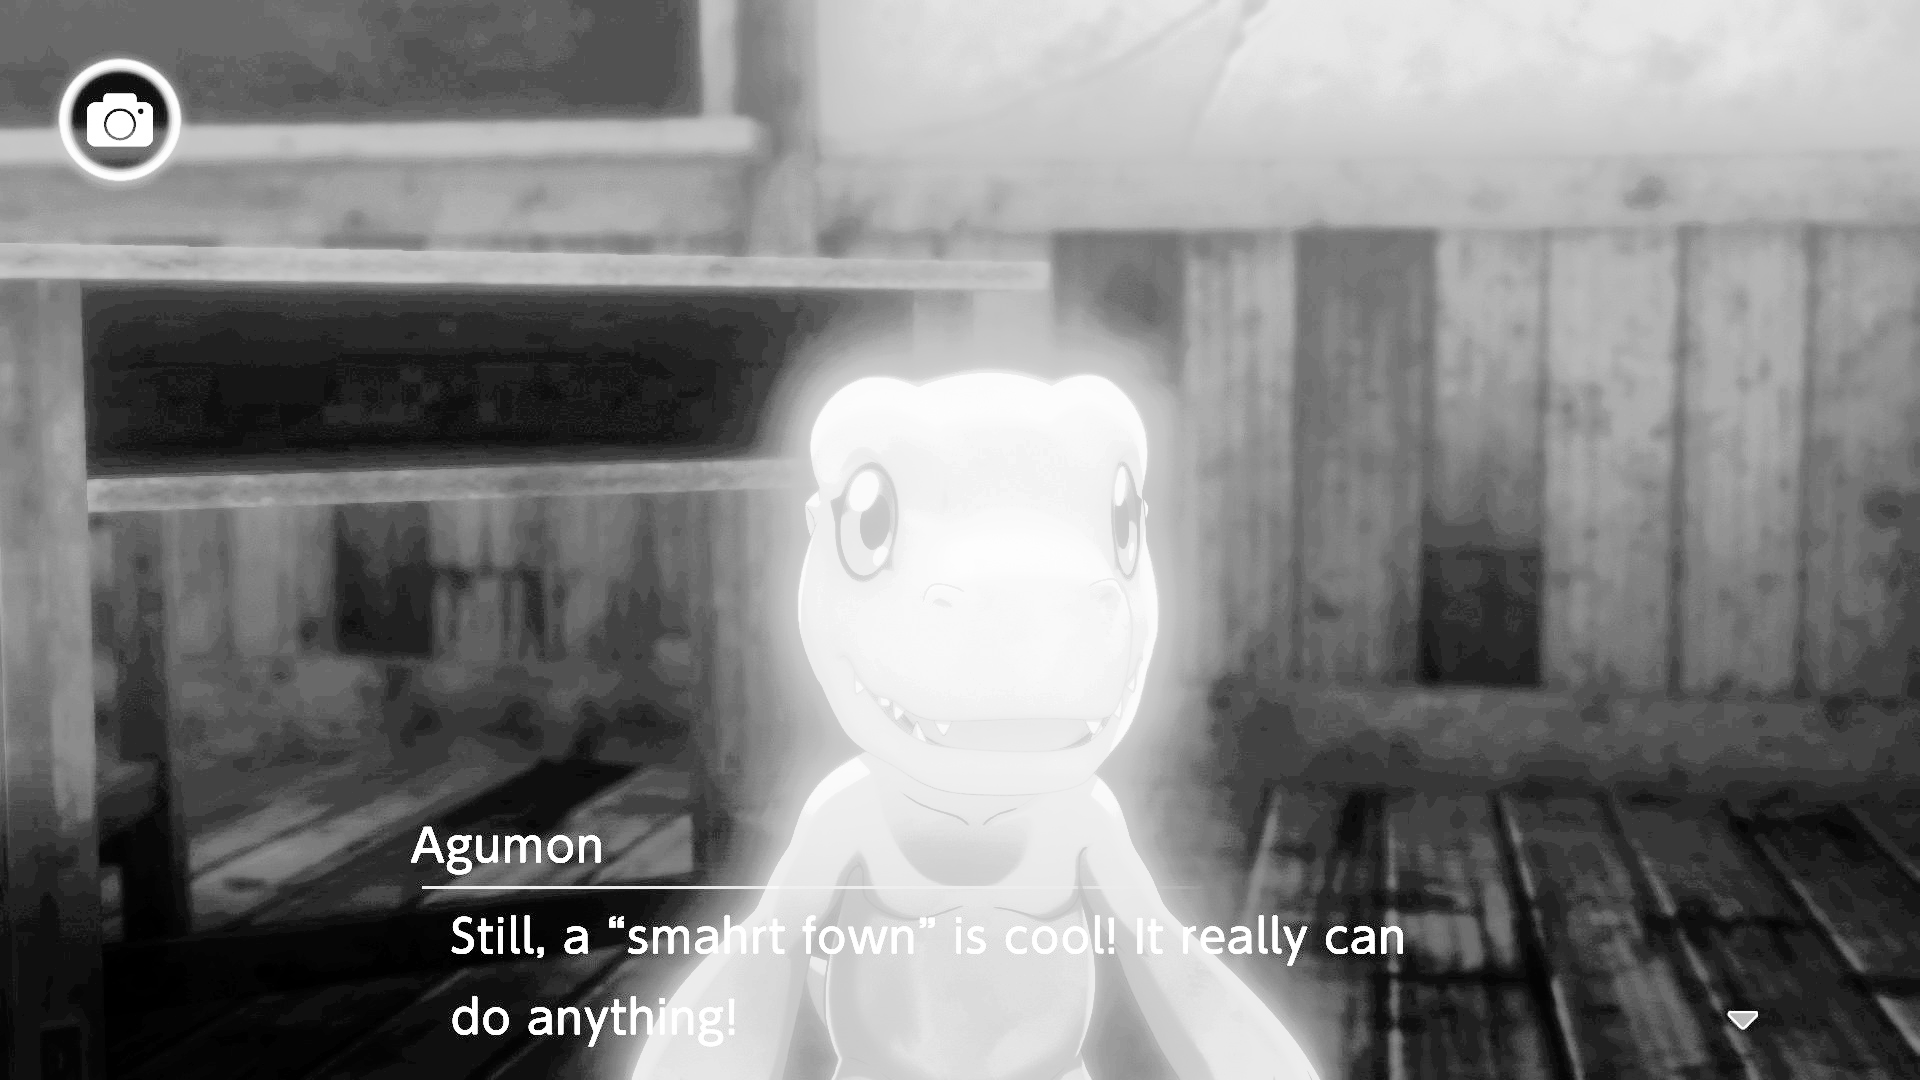
\includegraphics[width = 0.5\textwidth]{Imagenes/Preprocesado/3.png}
		\caption{Imagen con ecualización de histograma}
			\label{fig:Histograma}
	\end{figure}
	
	\item Corrección del gamma(Figura \ref{fig:Gamma}):
	Ajusta los valores de intensidad en la imagen para compensar la percepción humana y los errores del sensor, lo que puede hacer que ciertas áreas sean más visibles.
		\begin{figure}[H]
		\centering
		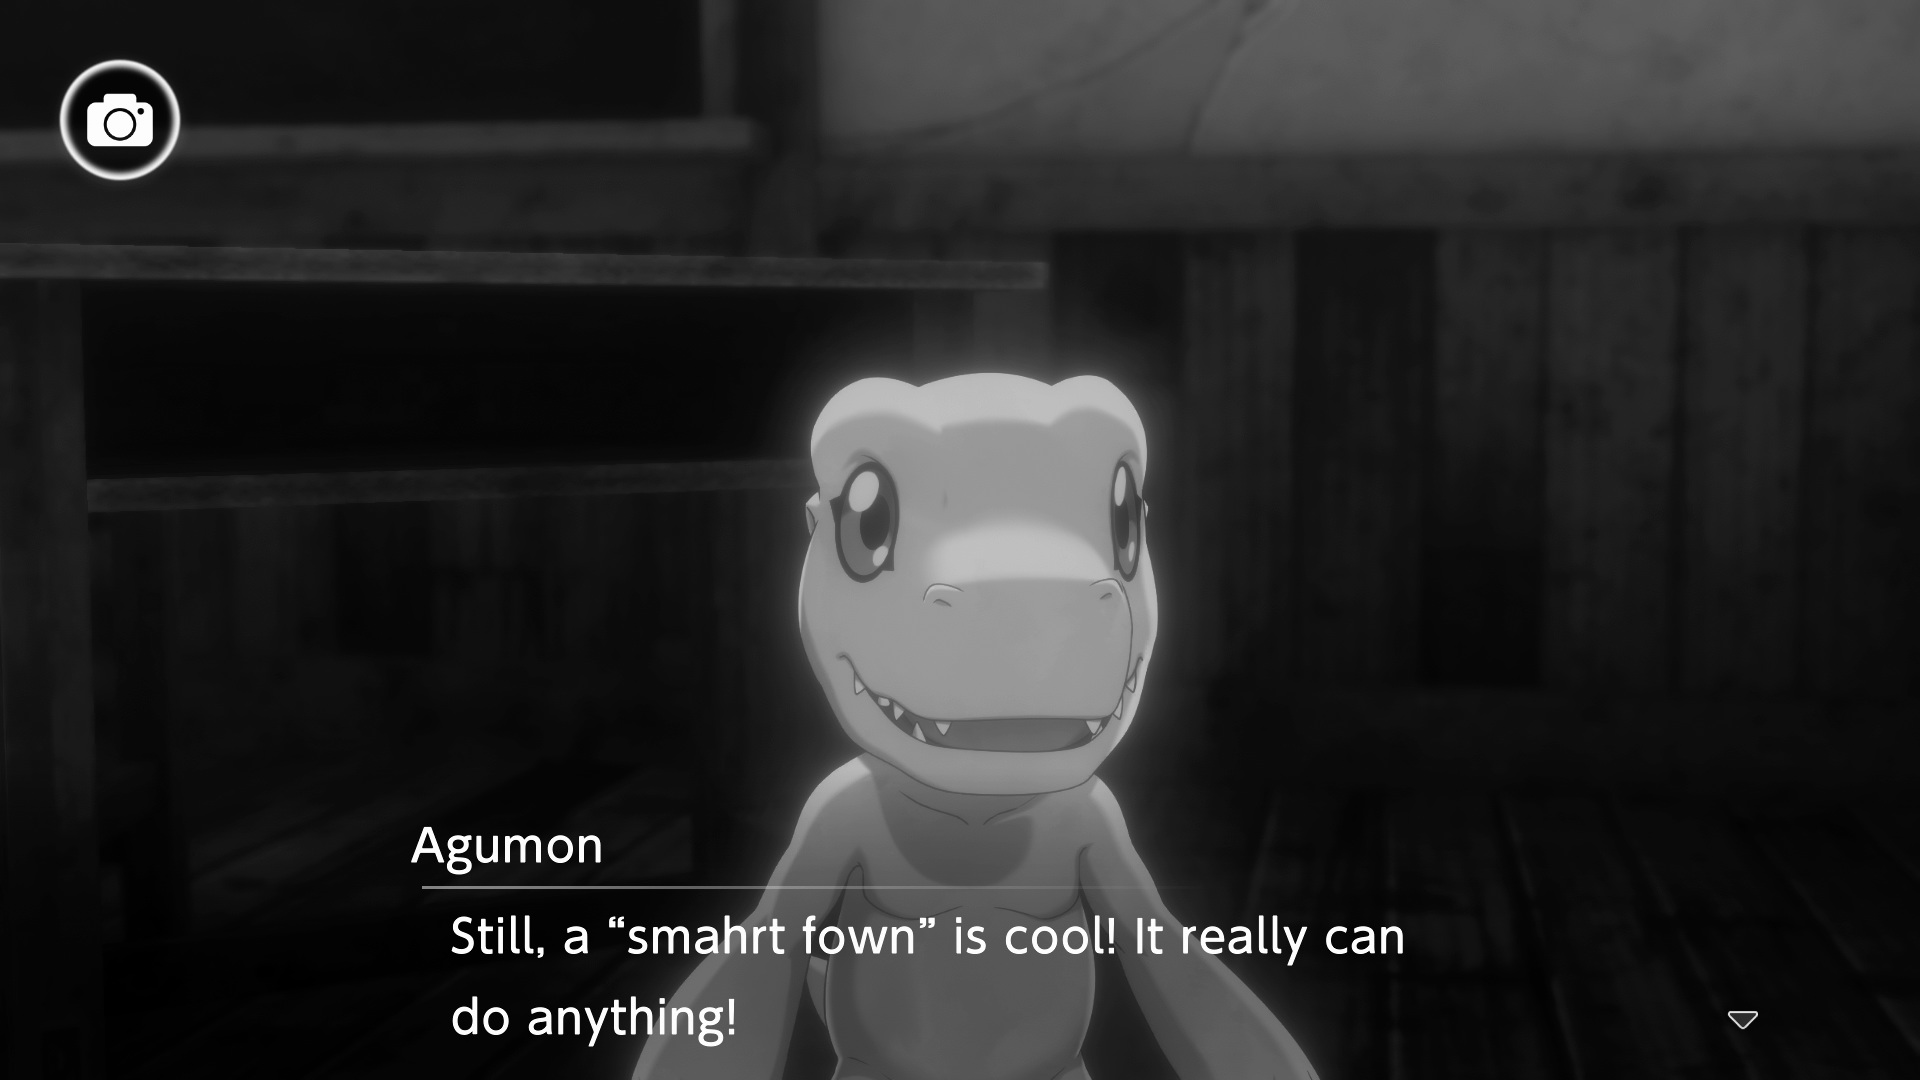
\includegraphics[width = 0.5\textwidth]{Imagenes/Preprocesado/4.png}
			\caption{Imagen con corrección del gamma}
			\label{fig:Gamma}
	\end{figure}
	
	\item Filtro de nitidez(Figura \ref{fig:F.Nitidez}): 
	Realza los bordes de una imagen para destacar detalles, útil en aplicaciones donde se requiere mayor definición.
		\begin{figure}[H]
		\centering
		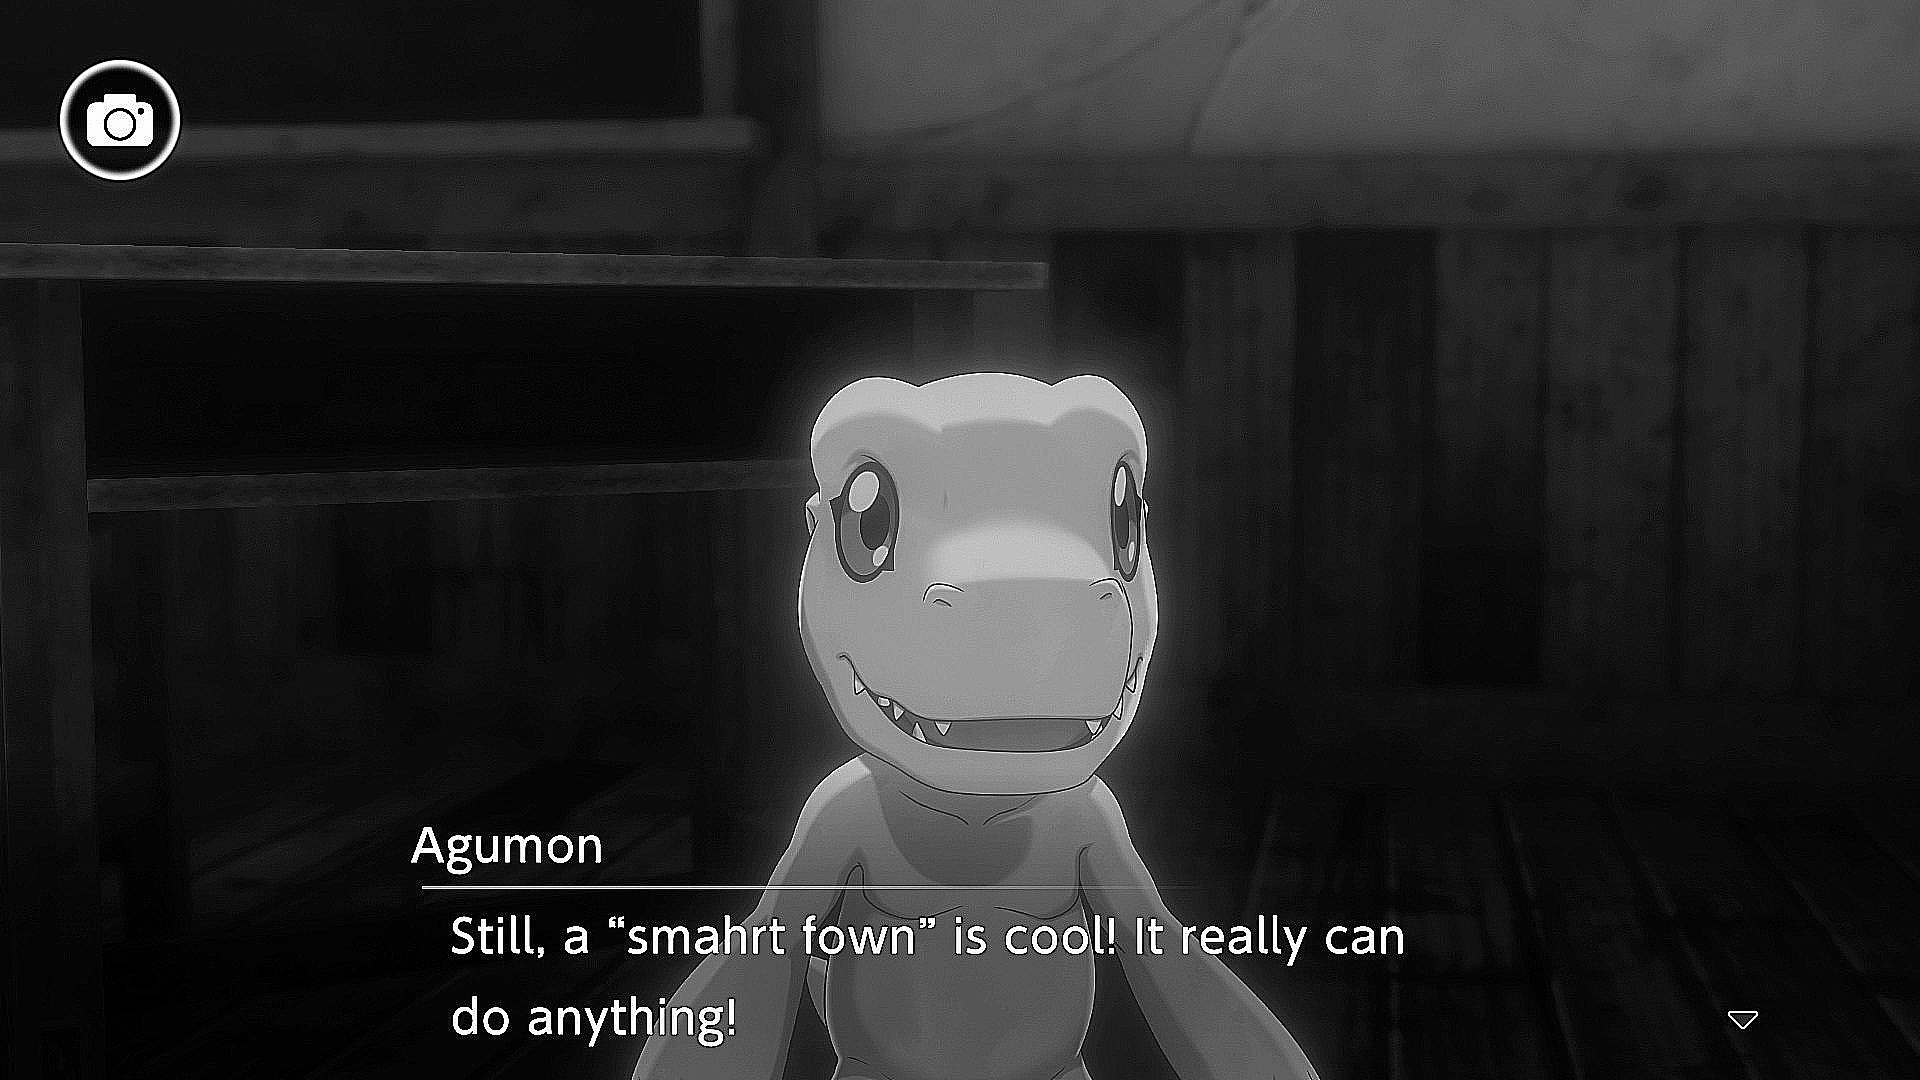
\includegraphics[width = 0.5\textwidth]{Imagenes/Preprocesado/5.png}
			\caption{Imagen con filtro de nitidez}
			\label{fig:F.Nitidez}
	\end{figure}
	
	\item Adaptive Thresholding(Figura \ref{fig:Thresholding}):
	Segmenta una imagen dividiéndola en áreas claras y oscuras, aplicando un umbral que se ajusta de forma adaptativa a las variaciones locales de luz.
		\begin{figure}[H]
		\centering
		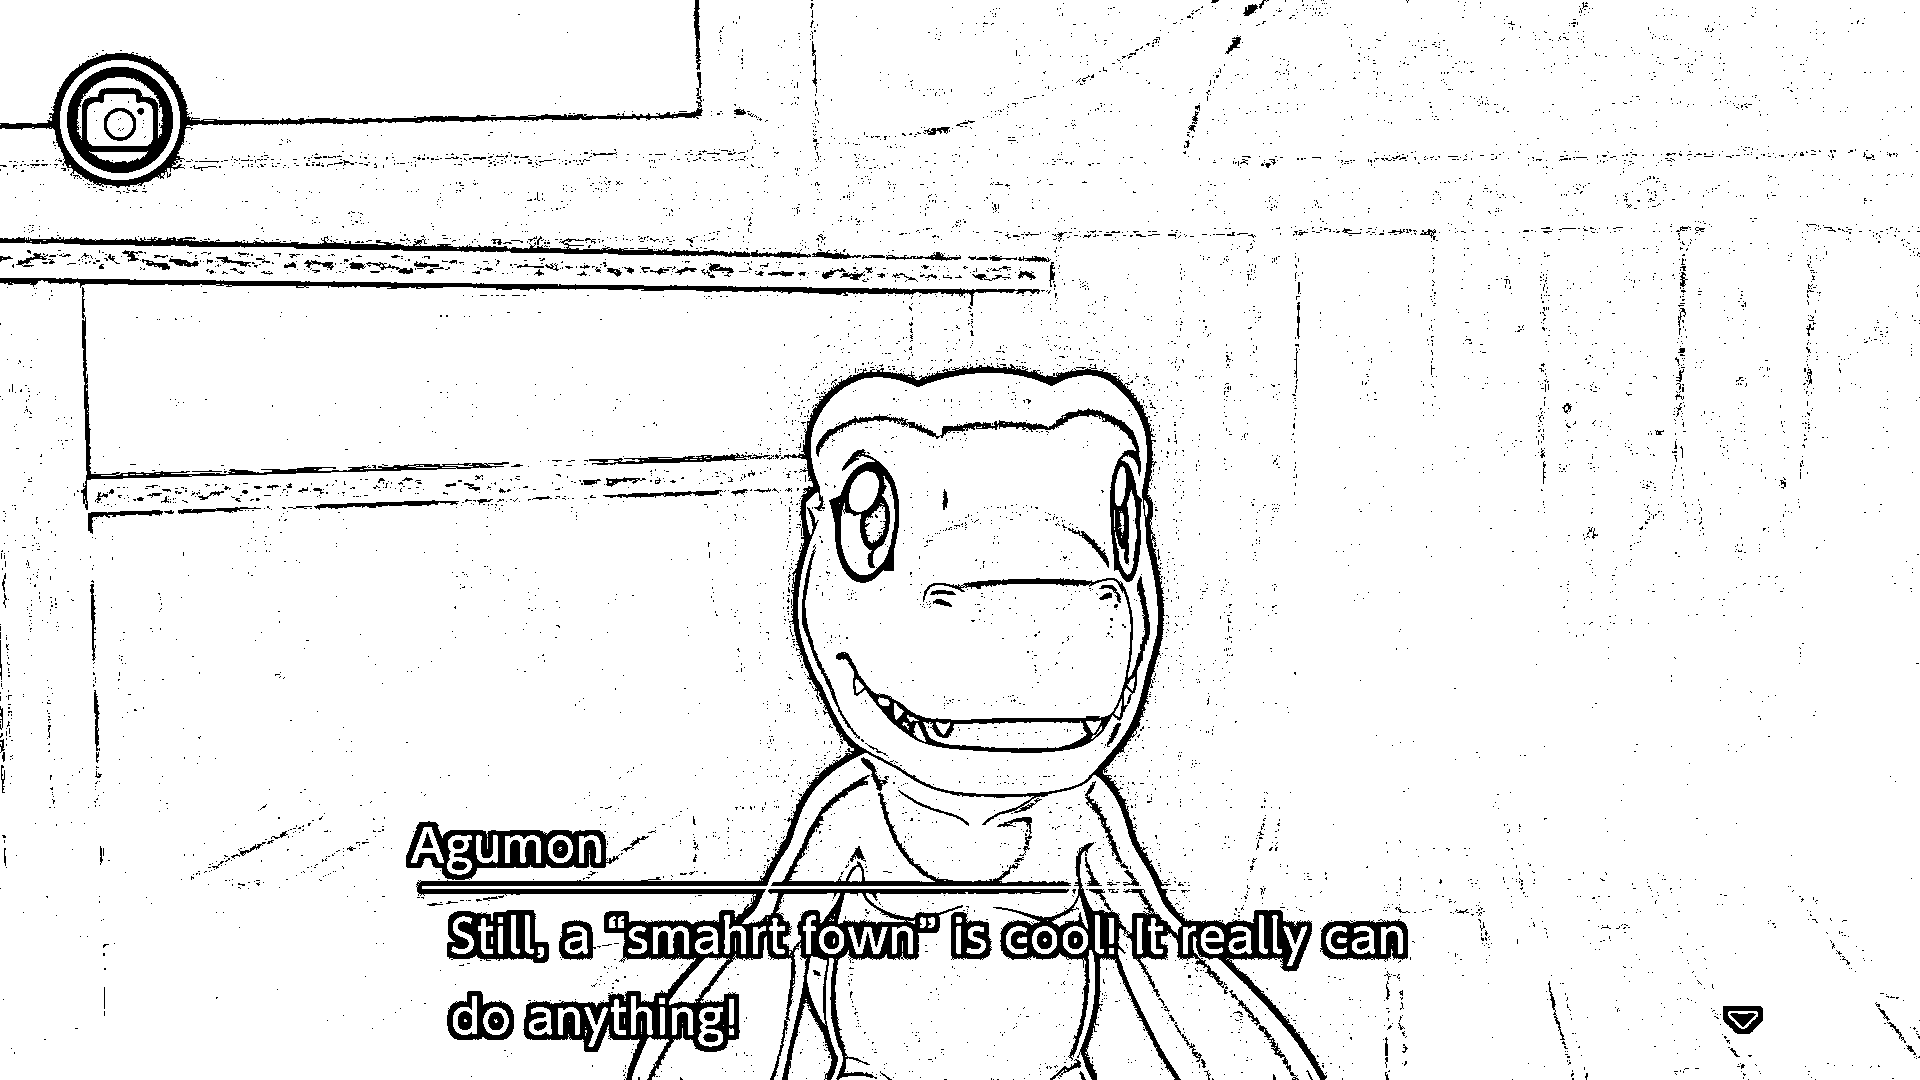
\includegraphics[width = 0.5\textwidth]{Imagenes/Preprocesado/6.png}
		\caption{Imagen aplicando adaptive thresholding}
			\label{fig:Thresholding}
	\end{figure}
	
	\item Simple Thresholding(Figura \ref{fig:S.Threshold}): 
	Asigna un valor binario a cada píxel dependiendo de si está por encima o por debajo de un umbral específico, útil para crear máscaras y segmentación sencilla.
		\begin{figure}[H]
		\centering
		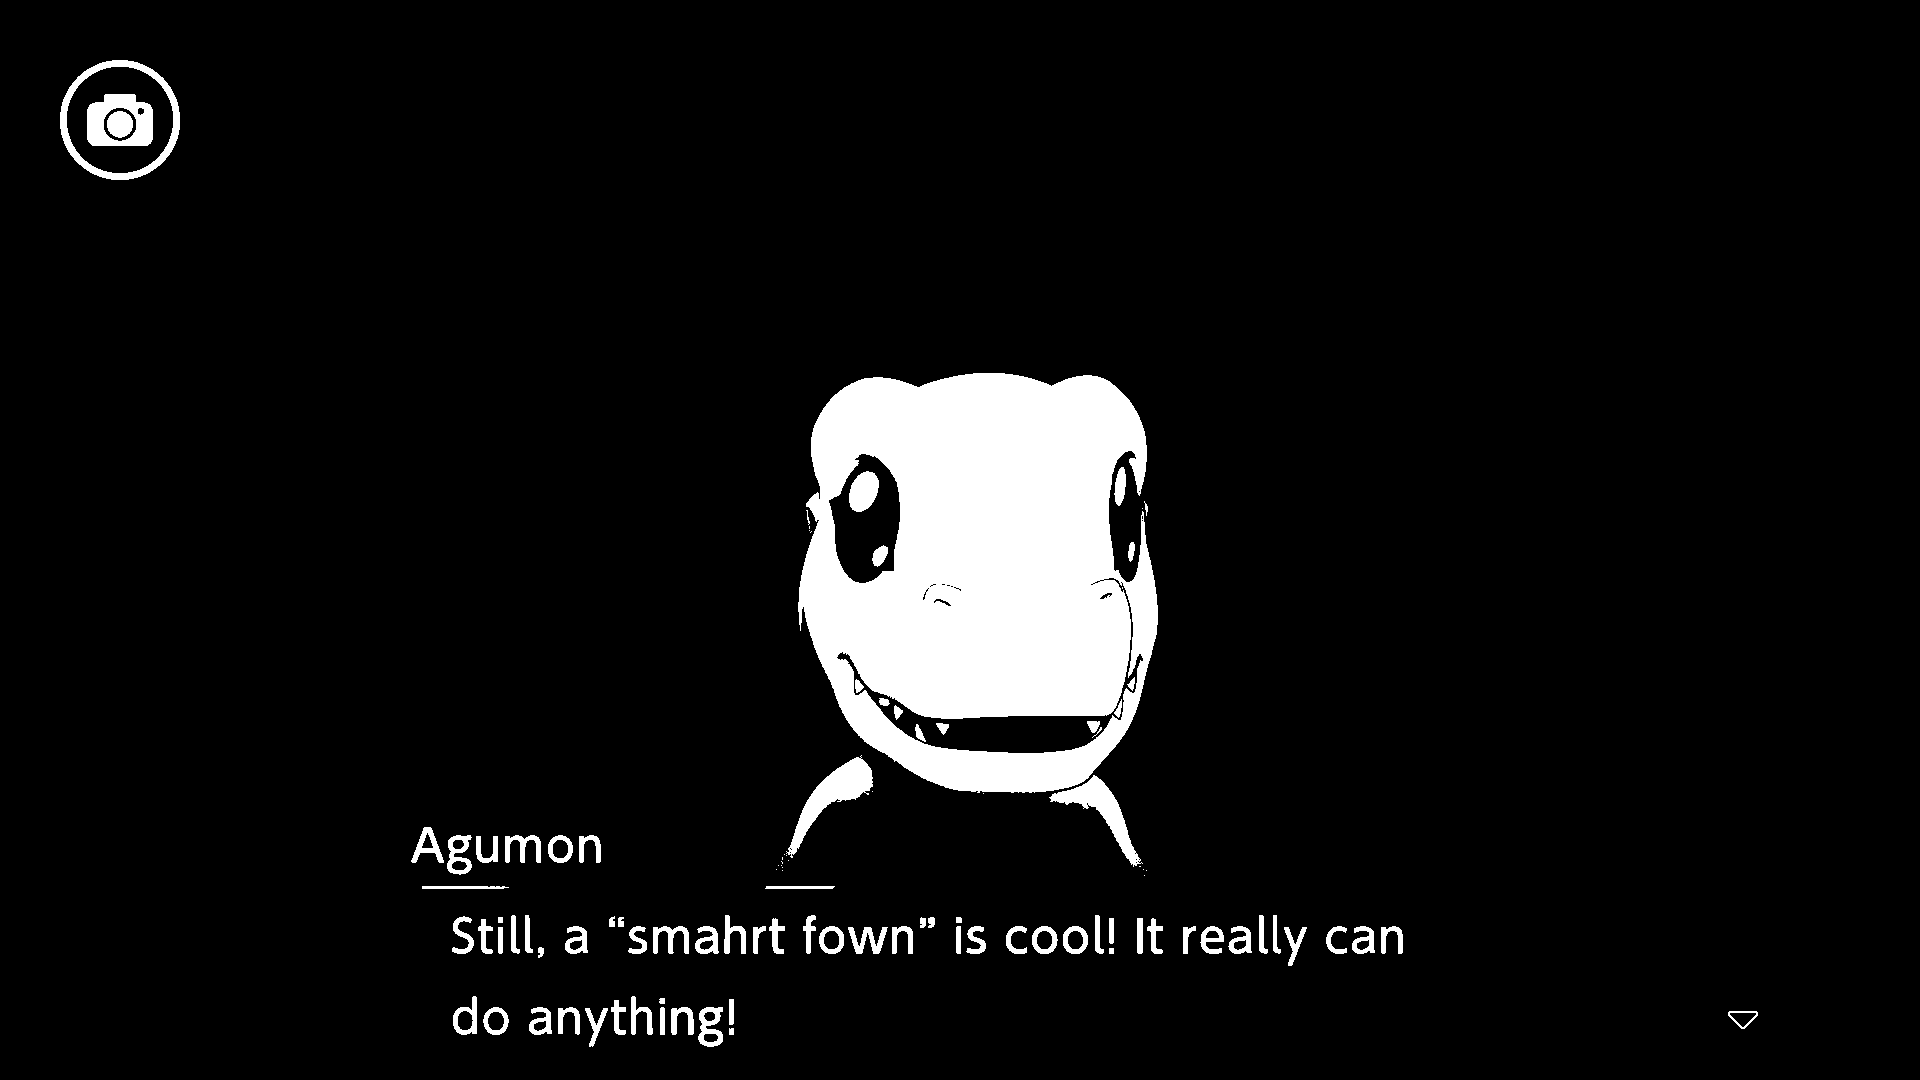
\includegraphics[width = 0.5\textwidth]{Imagenes/Preprocesado/7.png}
		\caption{Imagen aplicando simple thresholding}
		\label{fig:S.Threshold}
	\end{figure}
	
	\item Image Blurring (Desenfoque de Imagen)(Figura \ref{fig:Blurring}): 
	Reduce el ruido y los detalles mediante técnicas como filtros Gaussianos o de promediado, comúnmente utilizado para suavizar imágenes antes de un análisis.
		\begin{figure}[H]
		\centering
		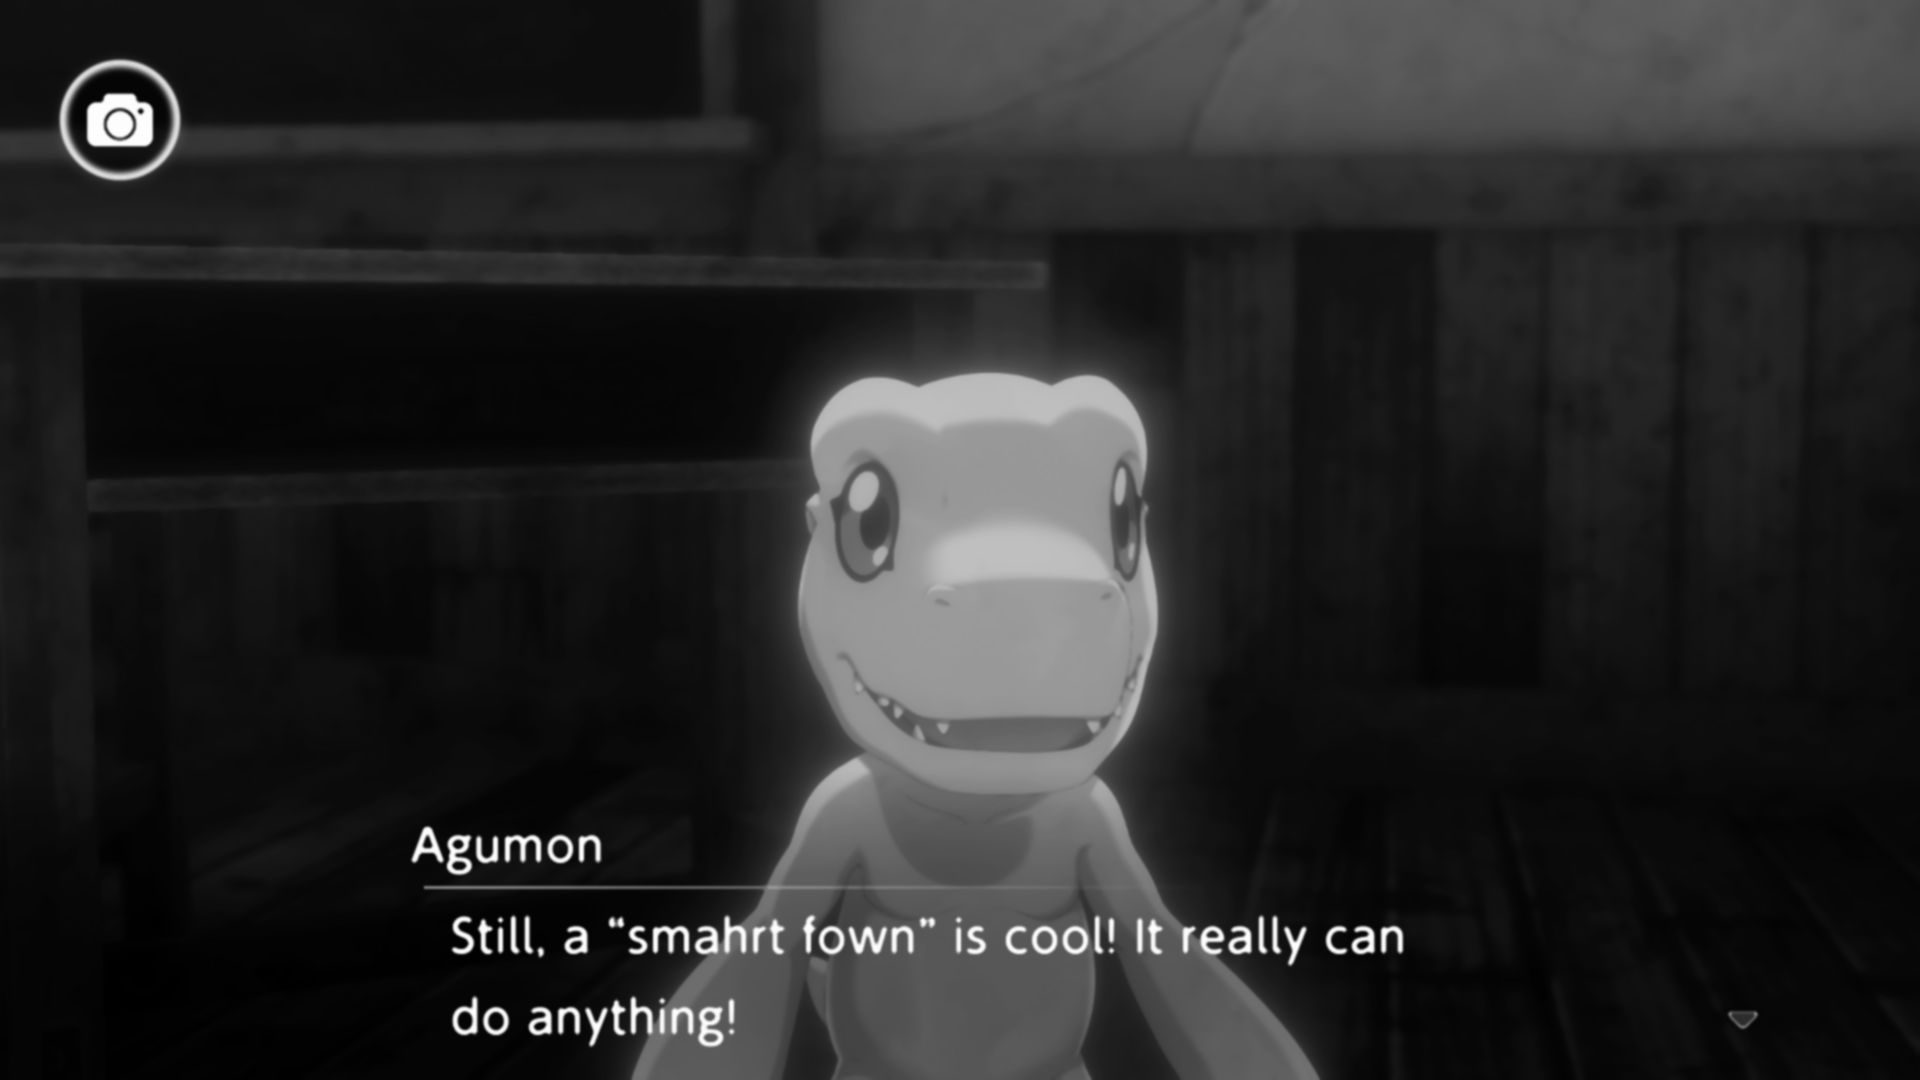
\includegraphics[width = 0.5\textwidth]{Imagenes/Preprocesado/8.png}
			\caption{Imagen aplicando desenfoque de imagen}
			\label{fig:Blurring}
	\end{figure}
	
	\item Redimensionar la imagen: 
	Cambia las dimensiones de una imagen, lo que puede ser útil para normalizar entradas a una red neuronal o ajustar el tamaño de una imagen para procesamiento.
		
	\item Dilatar y erosionar(Figura \ref{fig:Dilate_Erode}): 
	Técnicas de morfología matemática que expanden o reducen las regiones blancas (o los objetos) en una imagen binaria, útiles para limpieza de ruido o cierre de contornos.
		\begin{figure}[H]
		\centering
		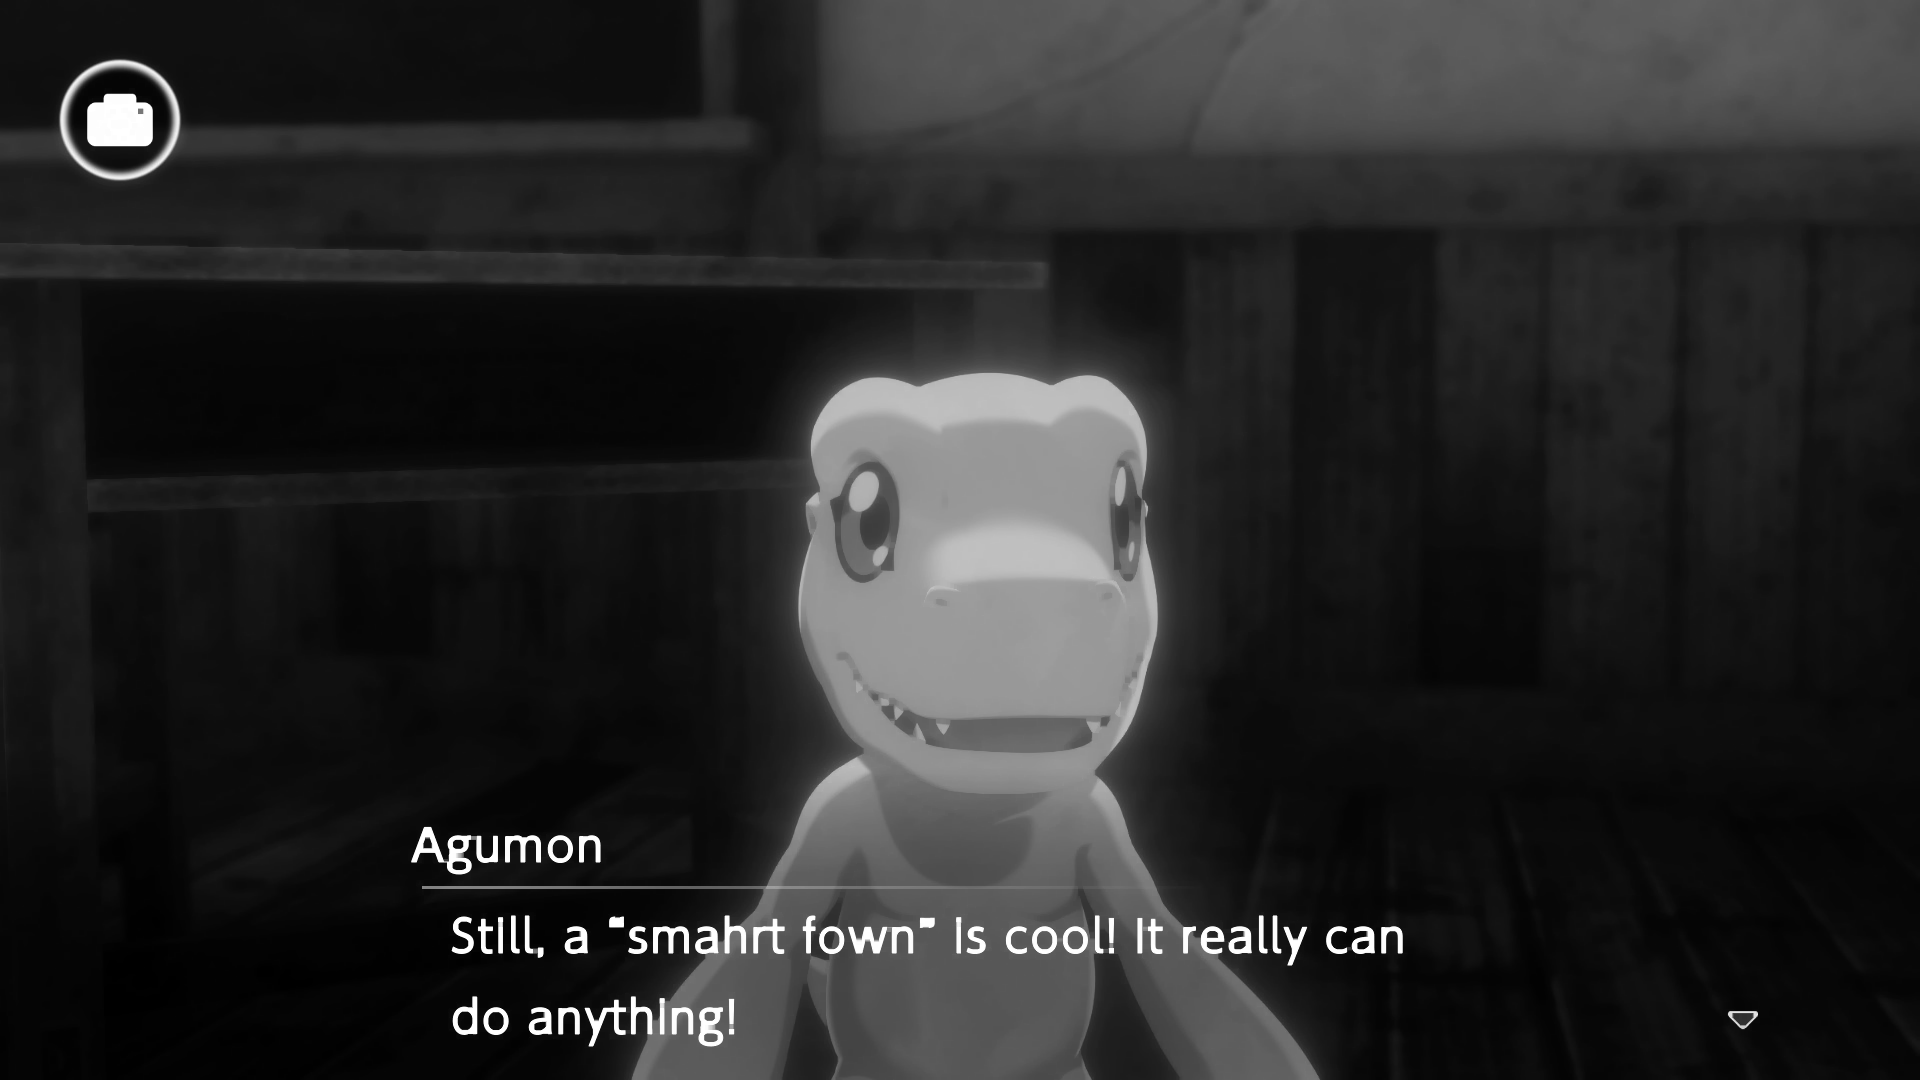
\includegraphics[width = 0.5\textwidth]{Imagenes/Preprocesado/10.png}
			\caption{Imagen dilatado y erosionado}
			\label{fig:Dilate_Erode}
	\end{figure}
	
	\item Denoising (Reducción de ruido)(Figura \ref{fig:Denoising}): 
	Elimina o reduce el ruido en una imagen para mejorar la calidad visual y el rendimiento de tareas de reconocimiento.
		\begin{figure}[H]
		\centering
		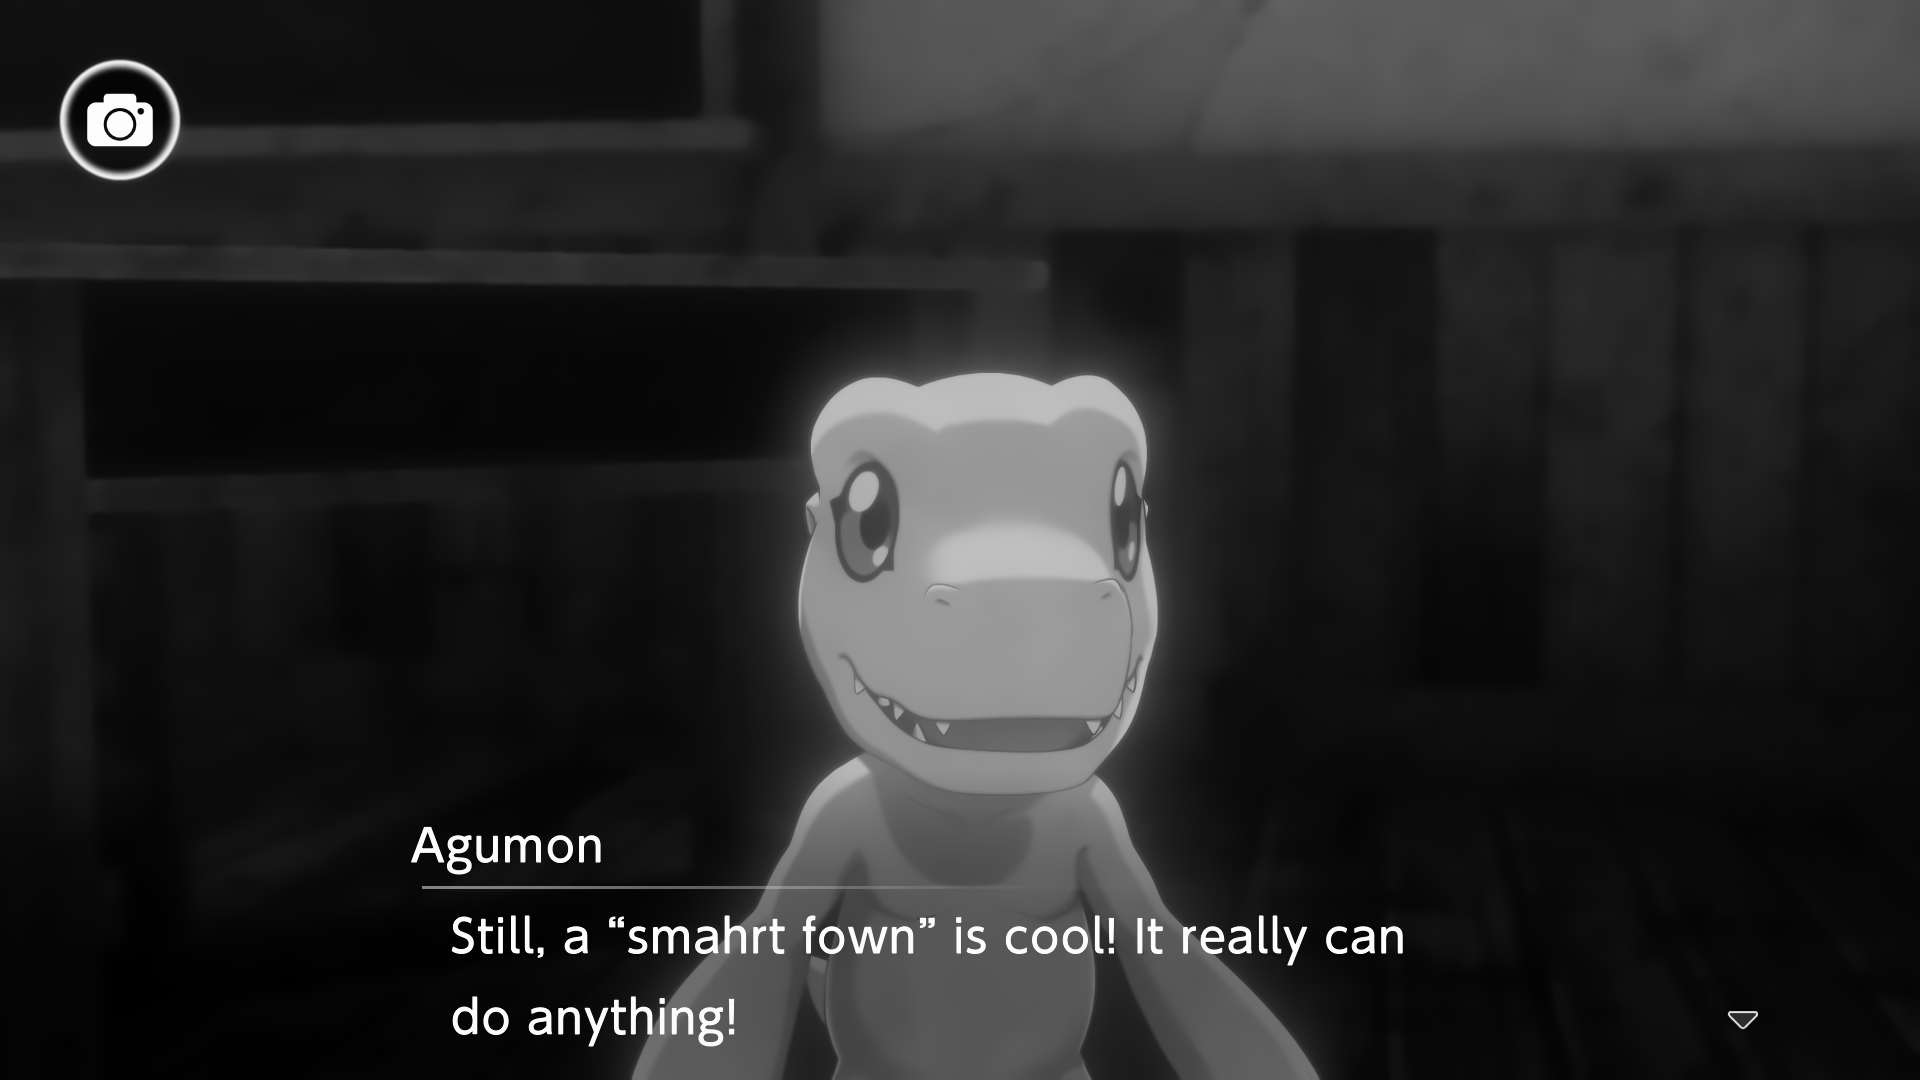
\includegraphics[width = 0.5\textwidth]{Imagenes/Preprocesado/11.png}
			\caption{Imagen aplicando reducción de ruido}
		\label{fig:Denoising}
	\end{figure}
	
\end{enumerate}
A continuación se ha hecho el experimento de aplicar un solo tipo de preprocesamiento a todas las imágenes de cada categoría, ejecutando el OCR sobre las imágenes preprocesadas y obteniendo el CER de cada imágen y el CER medio de cada categoría. Este proceso se ha aplicado para cada uno de las posibles técnicas de preprocesamiento obteniendo el resultado en la tabla \ref{table:preproCERtable}. Cada columna representa la categoría de la imagen y cada fila representa el preprocesamiento aplicado a las imágenes. En este caso no se hace distinción de OCR ya que preprocesamiento se aplica directamente en las imágenes antes de ser pasados a la OCR por lo que no importa la librería de OCR que se este usando.
Se marca en rojo aquel tipo de preprocesamiento que da peor resultado en la categoría y en verde, aquel que da mejor resultado.
\begin{table}[H]
	\begin{tabular}{llllll}
		Tipo                                                                 & F.Complejo                      & F.Simple                      & PixelArt                      & TxTBoc                       & TxtBoc2                       \\
			Nada                                                               & 9.39                          & 1.05                         & 2.51                          & 2.02                         & 5.61                          \\
		Grises                                                               & 3.72                          & 0.59                         & 2.69                          & 1.17                         & 2.16                          \\
		Contraste                                                            & 5.06                          & 0.81                         & 2.39                          & 1.13                         & 10.07                         \\
		\begin{tabular}[c]{@{}l@{}}Ecualización\\ de histograma\end{tabular} & 5.59                          & 3.60                         & 6.56                          & 2.41                         & 8.67                          \\
		Gamma                                                                & 3.72                          & 0.59                         & 2.69                          & 1.17                         & 2.16                          \\
		Filtro de nitidez                                                    & 11.06                         & 2.17                         & 8.84                          & 3.29                         & 12.05                         \\
		Thresholding C                                                       & \cellcolor[HTML]{FF0000}16.80 & \cellcolor[HTML]{FF0000}9.44 & 10.36                         & 4.08                         & \cellcolor[HTML]{FF0000}23.44 \\
		\begin{tabular}[c]{@{}l@{}}Thresholding\\ Gaussian\end{tabular}      & 12.85                         & 9.35                         & \cellcolor[HTML]{FF0000}16.16 & \cellcolor[HTML]{FF0000}4.71 & 22.83                         \\
		Thresold Binary                                                      & 4.05                          & \cellcolor[HTML]{00FF00}0.49 & 2.14                          & 1.79                         & 2.04                          \\
		\begin{tabular}[c]{@{}l@{}}Redimension\\ x1.5\end{tabular}           & 4.77                          & 0.80                         & 2.86                          & 1.27                         & 3.07                          \\
		Gaussian Blur                                                        & 3.02                          & 0.68                         & 2.34                          & 1.14                         & 1.86                          \\
		Median Blur                                                          & 2.75                          & 0.51                         & 2.75                          & 1.25                         & 1.37                          \\
		2 Blur                                                               & 2.26                          & 0.59                         & 2.15                          & 1.22                         & \cellcolor[HTML]{00FF00}1.09  \\
		Dilatación y erosión                                                 & 2.19                          & 0.51                         & 2.48                          & \cellcolor[HTML]{00FF00}0.69 & 1.83                          \\
		Dilatación                                                           & \cellcolor[HTML]{00FF00}1.80  & 0.62                         & \cellcolor[HTML]{00FF00}1.23  & 0.80                         & 5.53                          \\
		Erosión                                                              & 2.02                          & 1.00                         & 2.57                          & 0.82                         & 1.21                          \\
		Denoising                                                            & 3.23                          & 0.57                         & 2.64                          & 1.07                         & 1.70                         
	\end{tabular}
	\caption{Tabla con los resultados de CER medio de cada categoría de imágenes después de aplicar un tipo de preprocesamiento.}
	\label{table:preproCERtable}
\end{table}

Como podemos observar, en la mayoría de los preprocesamientos, los resultados mejoran en comparación con la de sin aplicar nada. Sin embargo, hay otros que empeoran, esto es debido a que el preprocesamiento ha marcado más las líneas y las geometrías por lo que el OCR reconozca más caracteres ``basura'' por lo que el CER supera a 1(reconoce más caracteres de los que hay en el ground-truth). Esto no significa que el OCR vaya ir a peor, puede que reconozca mejor el texto esperado pero añadiendo más basura que antes, algo que intentaremos resolver en el siguiente apartado. 

Obteniendo esta tabla y viendo los resultados de imágenes se ha ido probando distintas combinaciones de preprocesados de imágenes y se ha obtenido la siguiente combinación:
\begin{itemize}
	\item Grises
	\item Escalado
	\item Simple Threshold
	\item Denoising
	\item Blurring
	\item Dilate\_Erode	
\end{itemize}
Obteniendo estos resultados:
\begin{table}[H]
	\begin{tabular}{lllll}
		Complejo & Simple & PixelArt & TxTBoc & TxtBoc2                      \\
		2.57     & 0.29   & 2.01     & 1.01   & 1.49
	\end{tabular}
\end{table}
\subsection{Eliminación de caracteres basura}
Obteniendo el resultado de CER medio de los preprocesamientos(tabla \ref{table:preproCERtable}), podemos ver que se produce muchos números que superan al 1, esto significa que el OCR ha reconocido más caracteres de lo que hay en el ground-truth, todos esos caracteres que sobran son caracteres basura y el texto que necesitaremos estará en algunas de esas líneas. En esta sección intentaremos eliminar esos caracteres basura dejando solo lo necesario.
	\begin{figure}[H]
	\centering
	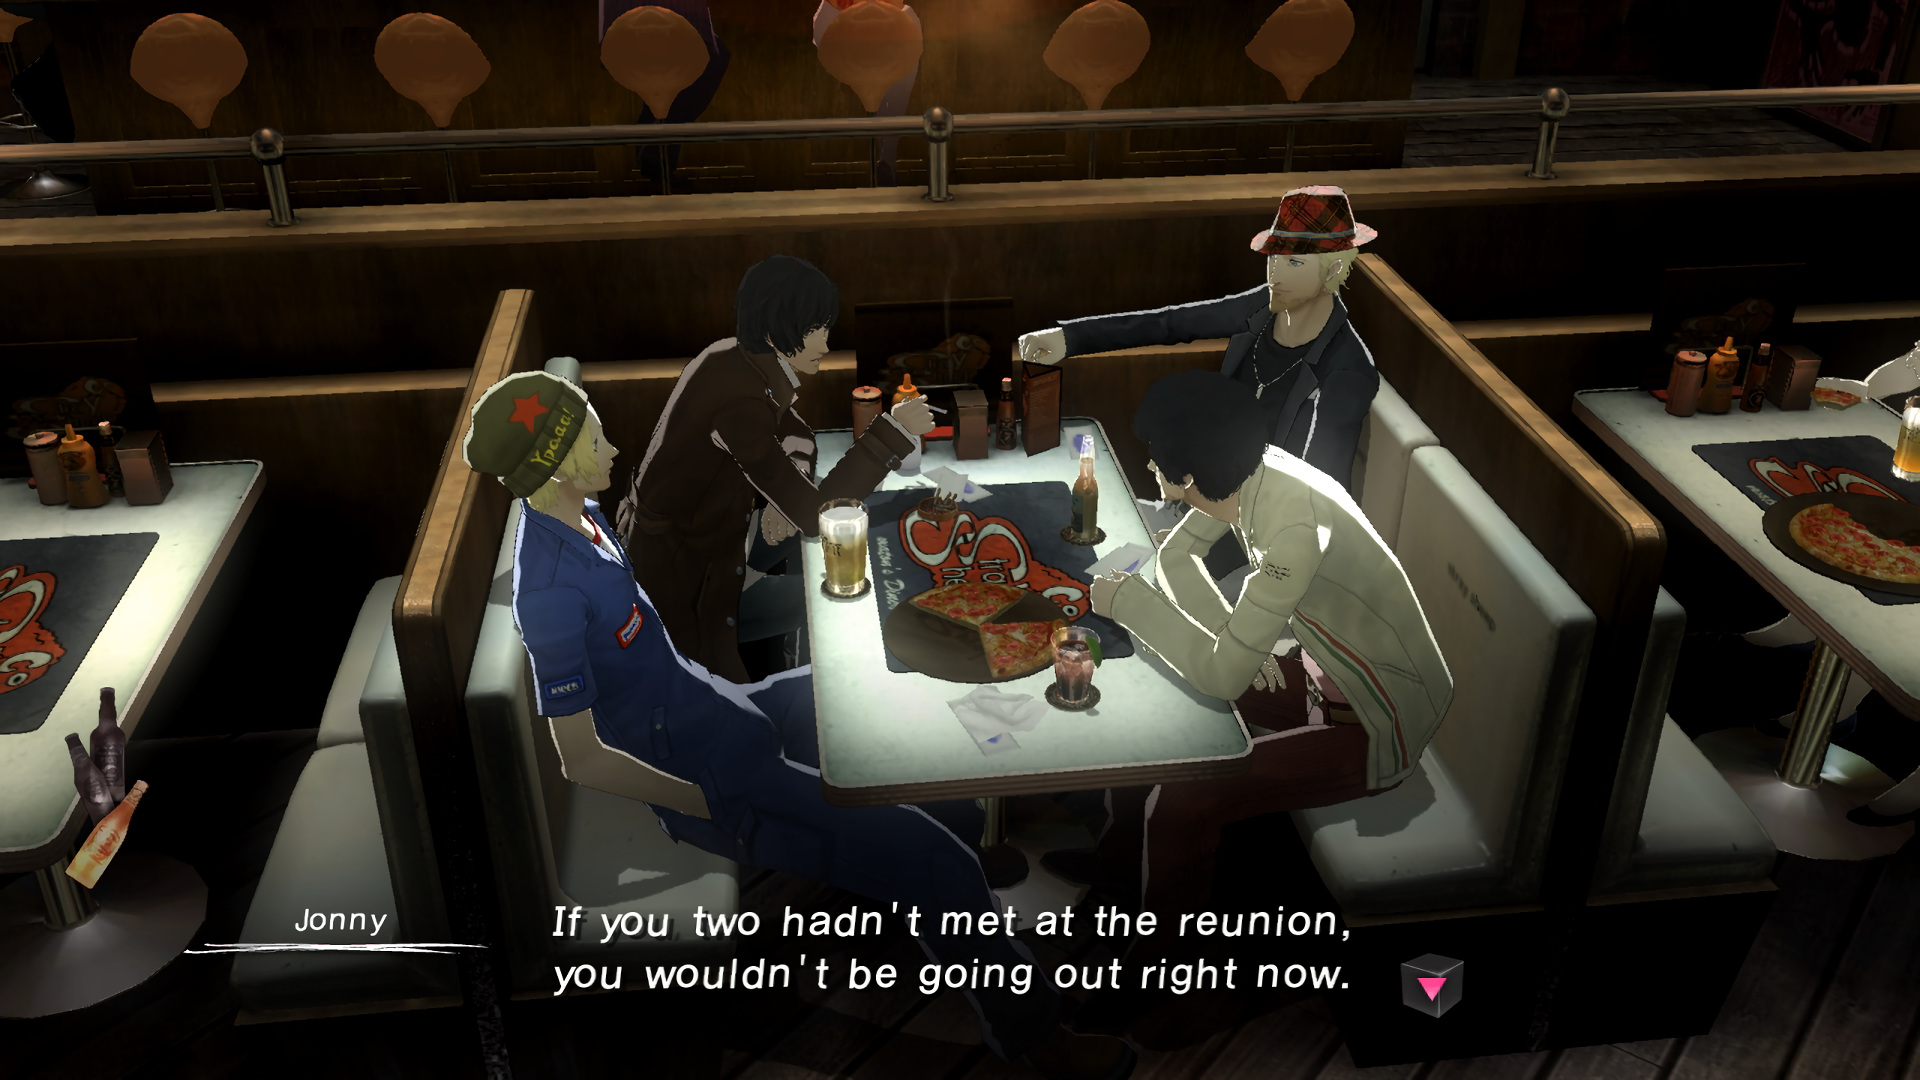
\includegraphics[width = 1\textwidth]{Imagenes/Sample_Trash_Char.png}
	\caption{Imagen ejemplo.}
	\label{fig:Trash_Char}
\end{figure}

El ground-truth de la figura \ref{fig:Trash_Char} es la siguiente:
\begin{verbatim}
	I - Under a New Sun
	Follow King Hugo
	AMICIA: It's been a long road. You have the right to strech your legs!
\end{verbatim}
Y una posible salida de la OCR con la figura \ref{fig:Trash_Char} puede ser la siguiente:
\begin{verbatim}
	ity L g i, ki " l i i e gl L i
	e "V‘m::::;:mw”,w"‘ M:u""% e m‘f L sl i 11 ff"».l,j, il fi’fw’“wn’hwiwm%‘» o i
	il TN e e S T it i i it o L i
	' g T g T i i e e Wt
	WS L ‘% s S o ‘m‘%‘ e S e i
	o i s N b i il e iR e e
	Mt “\nflfl‘_”"_m @M e, "m‘% il T s S il et :!,
	i — i Wl S e i i W il i ol il
	i o i, ‘:’? i W“‘gu | et il 'MW\ T
	e ; -"““ = = e = j - S
	5:2T"‘mw‘””“‘"““if., e, - WFM il i e, m S i
	i R g il i R g SR i i ca " "
	e " TR i iy o M y %} el b
	L e —— o —— usp—s
	i L " . o e x
	e : ST e i ol I ‘,“*'n‘ :
	T S ——— s i P, i R —— s
	B T W i e gL I e i g RPN — i ,":._.E_,Ev w-s—v* .
	e e ——a aEme TR
	e O e T M il e i i G il
	B i Wt 1t e »”‘1:\1'\WU}VHJ;\' i "[‘” A "'w;i A “fl”“”}}iuu” ‘f;;wx‘”HHHi‘i‘“ "}1"”‘HW\'W”‘“‘ i -
il Pfii'm”’”“‘iiimumu”wiilfll; e T M M e “‘H“"u . u” i 'miw:!!”l [ e I e
TR T e R " il e T R i il
R T e A i i S ! i e
T i “w:;‘:\!”::“‘\w L M e, T e o il M&rmzm,‘ i G T
MG T i g . o T e R S W i e
i L ‘ i il %v e U1 ":::hmwmmmw*“' P w:;-::;;:"" - e R Sy o e
e gy ~ e e R WWWV Bl g e i
‘ i s Wi i .““:;‘SY’"M||‘I“|IWWL .\"'“W"FTJC',':""'fiff“"m i :a’fl"“""!;w""’!"”Mfl?fl""fiwm.\-;,. 2 Iy " iy i
= el i S S VR S il o - T |
s e m*“fluflwj;"mrir%m iR e Wi - T D T e
s G e i g “"»;fi%.r}w!’w"flfiu,” om0 , ! i Mg W e e e I - ‘
e ‘!:;P‘":w‘w ‘"‘:"“""'v.v‘v‘-‘-‘-fs“ffifh:~“!‘“W;-':w" %’Wmmm%mflm e e 7 M,;“, o W M Dt e e N
£ .f, e A e M '}!{;‘;,:;:w:m..“,l“ V,»;%\YM"‘ G e I G
i i M L i By ..l T e e P (O, Ry i
e T s il e B N e =
ot e A ICIA: Iia b
i i m"""W- e ?‘q\;}‘;‘,‘.‘;!‘}:Mi«ximll‘nh\’lwwflfifl}y‘fimwm‘ e »‘:*Vn’(,fi, __nm:d e i = P — i
it A _-"J--m' 'A’mm__ “'.:I._'r;;;v e \mi‘w""' i “‘w e S o
R o T o
\end{verbatim}

Donde de forma subjetiva no encontramos ningún trozo del texto que se corresponda o sea parecido al ground-truth.

Después de aplicar el preprocesamiento elegido en el apartado anterior obtenemos el siguiente resultado:

\begin{verbatim}
	YRNY L., R Y .
	t ::;h.'. . ,’_:“?; -' [
	Y& i AT
	A DU T AR BIE
	e vl e \-' .: ’4 -7
	g ... . ‘s "
	_-'.‘_;g ""M“ a DO .
	* v o ‘ >
	e \1 v we » r
	—,:)‘“ - ~ ‘ S " v - .
	- ’ p S A ’ -t » e . -~
	) p '_" - Y . 4 ) ) e “ ",
	RS g~ C okl A e .
	o “\ ., ":.-.. _x '.- - — "- : ' . 1'1 N .»rv
	TN A foow. TREELYS 4 e
	v\ U - ' b.""*— .
	. . ) . ‘ . J - . h v ’k‘ Py
	Mo . : . ¢ . . . .
	. ’/. . A.; ‘-\ ' .
	it - g 03: b 4
	7 - ] > I »“ Y “. Pl
	L It's been a long road. You have the right to stretch your legs!
	L2 p
	’ - . r £ . R ¥ h N\
	y /’ - . J ’ ‘- - .i;" N
	
\end{verbatim}

En esta salida ya podemos reconocer que hay una línea que se corresponde con la salida que esperamos.
La frase que realmente importa es solamente una o dos líneas de la salida
\begin{verbatim}
		L It's been a long road. You have the right to stretch your legs!
\end{verbatim}
Esto es un problema importante que debemos solucionar ya que es imposible saber si un test es correcto o no con esta entrada.

En esta sección se propone una solución a este problema de caracteres ``basura'' usando el algoritmo de distancia \emph{levenshtein}.

La distancia de Levenshtein(también conocida como distancia de edición) según un articulo de \cite{LevDistance}, es una métrica utilizada para medir el grado de diferencia entre dos cadenas de texto. Específicamente, se define como el número mínimo de operaciones necesarias para transformar una cadena en otra, utilizando tres tipos de operaciones básicas:
\begin{itemize}
	\item Inserciones: Agregar un carácter.
	\item Eliminaciones: Eliminar un carácter.
	\item Sustituciones: Reemplazar un carácter por otro.
\end{itemize}

Suponiendo que tenemos el texto esperado de la imagen,  utilizando esta métrica, podemos obtener la distancia levenshtein entre una línea del texto esperado y una línea del texto reconocido por la OCR. Con la distancia obtenida y aplicando un cierto umbral, podemos identificar aquellas líneas que más se asimila al texto esperado, obteniendo así las líneas deseadas y descartando aquellas que no cumpla un cierto umbral.

Uno de los resultados obtenidos aplicando la distancia levenshtein es la siguiente si aplicamos un umbral de similitud de 0.8 (tiene que ser 80\% de parecido):
\begin{itemize}
		\item Texto real de OCR:
	\begin{verbatim}
		"
		|
		\ J
		—
		Agumon /
		Still, a “smahrt fown” is cool! It really can
		do anything! <
	\end{verbatim}
	\item Texto esperado:
	\begin{verbatim}
		Agumon
		Still,a "smahrt fown" is cool! It really can
		do anything!
	\end{verbatim}
	La fórmula general para calcular la similitud es:
	
	$Simulitud = 1-\frac{d}{max(s1,s2)} $ 
	
	Donde:
	
	\textit{d} es la distancia levenshtein.
	
	\textit{max(s1,s2)}	 es el máximo entre la longitud de la cadena \textit{s1} y cadena \textit{s2}
	
	Empezamos comparando la primera línea de OCR con la primera línea del esperado y así todo el rato hasta que comparemos todas.
	
	\item Texto aplicando distancia levenshtein:
	\begin{verbatim}
	Agumon /
	Still "smahrt fown" is cool! It really can 
	do anything! <
	\end{verbatim}
\end{itemize}  
Aplicando levenshtein a los resultados de todas las imágenes de cada categoría mencionadas en el apartado anterior después de aplicar preprocesamiento obtenemos estos nuevos resultados del CER medio de cada categoría:

\begin{table}[H]
	\begin{tabular}{llllll}
		Tipo        & Complejo & Simple & PixelArt & TxTBoc & TxtBoc2                      \\
		OCR         & 2.57     & 0.29   & 2.01     & 1.01   & \cellcolor[HTML]{FFFFFF}1.49 \\
		Levenshtein & 0.63     & 0.16   & 0.63     & 0.55   & 0.42                        
	\end{tabular}
\end{table}
El resultado de OCR es el resultado que obtenemos con solamente aplicando el preprocesamiento del apartado anterior. Sobre esa salida, se aplica la distancia levenshtein para la eliminación de basura obteniendo los nuevos resultados. Podemos ver en los números que mejoran casi un 50\% en todas la categorías por lo que es una técnica viable para nuestra herramienta.

 

